\documentclass{article}

% Language setting
% Replace `english' with e.g. `spanish' to change the document language
\usepackage[spanish]{babel}

% Set page size and margins
% Replace `letterpaper' with`a4paper' for UK/EU standard size
\usepackage[letterpaper,top=2cm,bottom=2cm,left=3cm,right=3cm,marginparwidth=1.75cm]{geometry}

% Useful packages
\usepackage{amsmath}
\usepackage[dvipsnames]{xcolor}
\usepackage{mwe}
\usepackage{datetime}
\usepackage{graphicx}
\usepackage{ amssymb }
\usepackage[colorlinks=true, allcolors=blue]{hyperref}
\usepackage{float}
%\usepackage{caption}
\usepackage{subcaption}
\usepackage{hyperref}
\usepackage{mathtools}
\usepackage[T1]{fontenc}
\usepackage{imakeidx}
\usepackage[font=small,labelfont=bf]{caption}
\DeclarePairedDelimiter\abs{\lvert}{\rvert}
%\title{Agujeros Negros de Kerr}
%\author{Guillermo Rodríguez Vega}
\newdateformat{monthyeardate}{\monthname[\THEMONTH], \THEYEAR}
\makeindex
\begin{document}

\begin{titlepage}
\begin{minipage}{\linewidth}
      \centering
      \begin{minipage}{0.45\linewidth}
          \begin{figure}[H]
              
\includegraphics[width=0.9\linewidth]{USC.png}
              
          \end{figure}
      \end{minipage}
      \hspace{0.05\linewidth}
      \begin{minipage}{0.45\linewidth}
          \begin{flushright}
            \large
            \color{Blue}
            FACULTAD DE FÍSICA\\GRADO EN FÍSICA\\curso 2021-22\\TRABAJO FIN DE GRADO
        \end{flushright}
      \end{minipage}
  \end{minipage}

\vspace{4cm}
\hrule
\vspace{1cm}

\centering
{\Huge AGUJEROS NEGROS DE KERR}
\vspace{2cm}
\hrule
\vspace{8cm}
\begin{flushleft}
\textit{Autor:}\\
\textbf{Rodríguez Vega, Guillermo}\\
\vspace{0.5cm}
\textit{Tutor:}\\
\textbf{Álvarez Muniz, Jaime}\\ 
Área de Física Teórica, Departamento de Física de Partículas.
\end{flushleft}
\begin{flushright}
\monthyeardate\today
\end{flushright}
\end{titlepage}

\tableofcontents

\begin{abstract}
 
\end{abstract}
\renewcommand{\abstractname}{Resumo}
\begin{abstract}
 
\end{abstract}
\renewcommand{\abstractname}{Abstract}
\begin{abstract}
 
\end{abstract}

\section{Introducción}
Un agujero negro es el colapso gravitatorio de una cierta cantidad de masa, se producen cuando una estrella pierde el equilibrio hidrostático en favor de la gravedad, por la conservación del momento angular si la estrella que dio origen al agujero negro tenía momento angular no nulo entonces el agujero negro tendrá también un momento angular, convirtiéndose en un agujero negro de Kerr.

\subsection{Breve introducción a Relatividad General}
La relatividad general se basa en dos postulados, la universalidad de la gravitación y el principio de equivalencia\cite{sarbach2011relatividad}. 

La universalidad de la gravitación dice que el movimiento de un cuerpo de prueba en un campo gravitacional es independiente de su masa o composición (despreciando las interacciones del espín y del momento cuadrupolar de la partícula con el campo gravitacional).\cite{sarbach2011relatividad}

El principio de equivalencia establece que en un campo gravitacional arbitrario, ningún experimento local puede distinguir un sistema en caída libre no-rotante (un sistema inercial local) de un sistema en movimiento uniforme en la ausencia de un campo gravitacional.\cite{sarbach2011relatividad}

El principio de equivalencia llevo a Einstein a pensar en la gravedad como la curvatura del espacio tiempo en lugar de una fuerza de atracción como podía ser el electromagnetismo.

\subsection{Ecuaciones de Einstein}
Por el principio de universalidad tenemos que la ecuación debe ser válida en todos los sistemas de referencia y que por lo tanto debe tener una forma tensorial de esta forma:\cite{janssen2013teoria}

\begin{equation}
    G_{\mu \nu}=-kT_{\mu \nu}
\end{equation}

Donde $G_{\mu \nu}$ es el tensor curvatura y $T_{\mu \nu}$ es el tensor momento-energía, mientras que k es una constante. La curvatura del espacio viene dada por la masa que contiene por lo que debe ser proporcional a ella.

El tensor curvatura $G_{\mu\nu}$ debe cumplir las siguientes propiedades\cite{janssen2013teoria}:

\begin{enumerate}
    \item Tiene que ser simétrico en los dos índices, ya que $T_{\mu\nu}$ también lo es.
    \item $G_{\mu\nu}$ tiene que ser un objeto puramente geométrico. Por lo tanto, tiene que ser una función
    solamente de la métrica $g_{\mu\nu}$ y sus derivadas.
    \item Para el espacio plano, tenemos que $G_{\mu\nu} = 0$.
    \item La ley de conservación de energía $\Delta_{\mu}T_{\mu\nu}= 0$ implica que también $\Delta_{\mu}G_{\mu\nu}= 0$.
    \item Se puede identificar la componente $g_{00}$ de la métrica con el potencial gravitacional newtoniano . Para tener una teoría dinámica y para recuperar la ecuación de Poisson, $G_{\mu\nu}$ debe contener segundas derivadas de la métrica. La manera mas
    natural, por lo tanto es a través de las contracciones del tensor de Riemann $R_{\mu\nu\rho}^{\lambda}$.
    \item Para obtener una ecuación diferencial de segundo orden (y no mas) en los potenciales gravitatorios, $G_{\mu\nu}$ tiene que ser lineal en el tensor de Riemann. Contracciones del tipo $R_{\mu\rho}R_{\nu}^{\rho}$ ó $R_{\mu\rho\lambda\sigma}R_{\nu}^{\rho\lambda\sigma}$ darían lugar a ecuaciones diferenciales de orden mas alto que 2.
\end{enumerate}

Siguiendo estas condiciones nos queda un tensor curvatura bastante bien definido:

\begin{equation}
    G_{\mu \nu}=R_{\mu \nu}-\frac{1}{2}g_{\mu \nu}R
\end{equation}

Una comparación con las fórmulas newtonianas fija la constante de proporcionalidad como $k=8\pi G_{N}$ \cite{janssen2013teoria}, entonces:

\begin{equation}
    G_{\mu \nu}=-8\pi  G_{N}T_{\mu \nu}
\end{equation}

Las ecuaciones de einstein vienen dadas entonces por:

\begin{equation}
    R_{\mu \nu}-\frac{1}{2}g_{\mu \nu}R=-8\pi  G_{N}T_{\mu \nu}
\end{equation}

\subsection{Solución de Schwarzschild y agujeros negros}

La solución de Schwarszchild es la solución de las ecuaciones de campo en el vacío, esta describe el campo gravitacional generado por un objeto masivo, estático, con simetría esférica y asintoticamente plano.\cite{rodriguez2019solucion}

Al estar en el vacío tenemos que el tensor momento-energía es nulo $T_{\mu \nu}=0$ y al multiplicar el tensor de Ricci por la métrica $g_{\mu \nu}$ obtenemos que las ecuaciones a resolver son:

 \begin{equation} \label{vacio}
     R_{\mu \nu}=0
 \end{equation}
 
La solución debe ser estática y tener simetría esférica por lo que:

\begin{equation}
    ds^{2}=
    -A(r)dt^{2} 
    +B(r)dr^{2} 
    +r^{2}d\Omega^{2}
\end{equation}

Las distintas componentes del tensor de Ricci quedan así:

\begin{enumerate}
    \item $R_{tt}=\frac{A''}{2B}+\frac{A'}{rB}-\frac{A'}{4B}\left(\frac{A'}{A}+\frac{B'}{B}\right)$
    \item $R_{rr}=-\frac{A''}{2B}+\frac{A'}{rB}+\frac{A'}{4B}\left(\frac{A'}{A}+\frac{B'}{B}\right)$
    \item $R_{\theta\theta}=1-\frac{1}{B}-\frac{r}{2B}\left(\frac{A'}{A}-\frac{B'}{B}\right)$
    \item $R_{\phi\phi}=sen^{2}\theta R_{\theta\theta}$
    \item El resto son nulos.
\end{enumerate}

Todos deben cumplir la condición (\ref{vacio}):
\begin{equation}
    \frac{R_{tt}}{A}+\frac{R_{rr}}{B}=0
\end{equation}

\begin{equation}
    \frac{A'}{rAB}+\frac{B'}{rB^{2}}=0
\end{equation}

\begin{equation}
    \frac{A'}{A}+\frac{B'}{B}=0
\end{equation}

\begin{equation}
    \ln(AB)=cte
\end{equation}
Pero sabemos que la solución de Schwarzschild tiene que ser un espacio plano en el limite $r \xrightarrow[]{} \infty$, entonces $A(r \xrightarrow[]{} \infty)=B(r \xrightarrow[]{} \infty)=1$, por lo tanto la constante cte=0, entonces $AB=1$.

También podemos considerar la ecuación $R_{\theta \theta}=0$ y que $AB=1$:

\begin{equation}
    1-A-rA'=0
\end{equation}
Resolviendo la ecuación diferencial queda:
\begin{align}
    A(r)=1+\frac{C}{r} && B(r)=\left( 1+\frac{C}{r}\right)^{-1}
\end{align}
Para obtener la constante de integración C basta con considerar que a grandes distancias, en el limite newtoniano; $g_{tt}=A(r)=1+2\phi(r)$\cite{rodriguez2019solucion} donde $\phi$ es el potencial de Newton $\phi=-M/r$, la constante de integración queda entonces $C=-2M$.

\begin{equation}
    ds^{2}=
    -\left(1-\frac{2M}{r}\right)dt^{2} 
    +\left(1-\frac{2M}{r}\right)^{-1}dr^{2} 
    +r^{2}d\theta^{2}+ 
    r^{2}sen^{2}\theta d\phi^{2}
\end{equation}

Para obtener la trayectoria de las partículas en la métrica de Schwarzschild debemos buscar la geodésica de esta métrica, que sería la trayectoria de esa partícula, teniendo siempre presente que la masa de la partícula es tan pequeña respecto a la de la “estrella” que se puede anular su aportación a la métrica del espacio. Para eso:\cite{zamorageodesicas}

\begin{equation}
    \mathcal{L}=g_{ij}\dot x^{i}\dot x^{j}=-1
\end{equation}

Que corresponde a:\cite{zamorageodesicas}

\begin{equation}\label{LagrangeS}
    \mathcal{L}=\left(1-\frac{2M}{r}\right)^{-1}\dot r^{2}+r^{2}sen^{2}\theta \dot \phi^{2}+r^{2}\dot \theta^{2}-\left(1-\frac{2M}{r}\right) \dot t^{2}=-1
\end{equation}

Sabiendo que las ecuaciones de Lagrange son:\cite{zamorageodesicas}

\begin{equation}
    \frac{d}{d\tau}\left(\frac{\partial \mathcal{L}}{\partial \dot x^{i}}\right)-\frac{\partial \mathcal{L}}{\partial \dot x^{i}}=0
\end{equation}

Obtenemos las ecuaciones:\cite{zamorageodesicas}

\begin{align}\label{ecsLagrangeS}
    \dot \theta=0 && r^{2}sen^{2}\theta \dot \phi=l && \dot t\left(1-\frac{2M}{r}\right)=e
\end{align}

Como $\theta$ es constante podemos suponer que estamos en el plano ecuatorial, $\theta=\pi/2$, sustituyendo (\ref{ecsLagrangeS}) en (\ref{LagrangeS}), obtenemos:\cite{zamorageodesicas}

\begin{equation}\label{MovSr}
    \frac{e^{2}-1}{2}=\frac{1}{2}\dot r^{2}+\left[ \frac{-M}{r}+\frac{l^{2}}{2r^{2}}-\frac{M l^{2}}{r^{3}}\right]
\end{equation}

Donde podemos interpretar $\mathcal{E}=\frac{e^{2}-1}{2}$ como la energía y lo que hay entre corchetes como el potencial efectivo:\cite{zamorageodesicas}

\begin{equation}
    V_{efe}(r)= \frac{-M}{r}+\frac{l^{2}}{2r^{2}}-\frac{M l^{2}}{r^{3}}
\end{equation}

Conociendo las ecuaciones del movimiento podemos representar las órbitas resolviendo las ecuaciones diferenciales numéricamente.\cite{zamorageodesicas}

Si usamos $\frac{dr}{d\tau}=\frac{dr}{d\phi}\frac{d\phi}{d\tau}$ en (\ref{MovSr}) y sustituyendo $r=1/u$, obtenemos:\cite{zamorageodesicas}

\begin{equation}
    \left(\frac{du}{d\phi}\right)^{2}-\frac{2Mu}{l^{2}}+u^{2}-2Mu^{3}-\frac{2\mathcal{E}}{l^{2}}
\end{equation}

Si ahora derivamos de nuevo respecto de $\phi$, considerando que $\left(\frac{d u}{d\phi}\right)\neq0$:\cite{zamorageodesicas}

\begin{equation}\label{MovSu}
    \frac{d^{2}u}{d^{2}\phi}=3Mu^{2}-u+\frac{M}{l^{2}}
\end{equation}

Podemos analizar numéricamente esta ecuación (\ref{MovSu}) utilizando un Runge-Kutta de orden 4.
\begin{figure}[H]
\begin{subfigure}{0.5\textwidth}
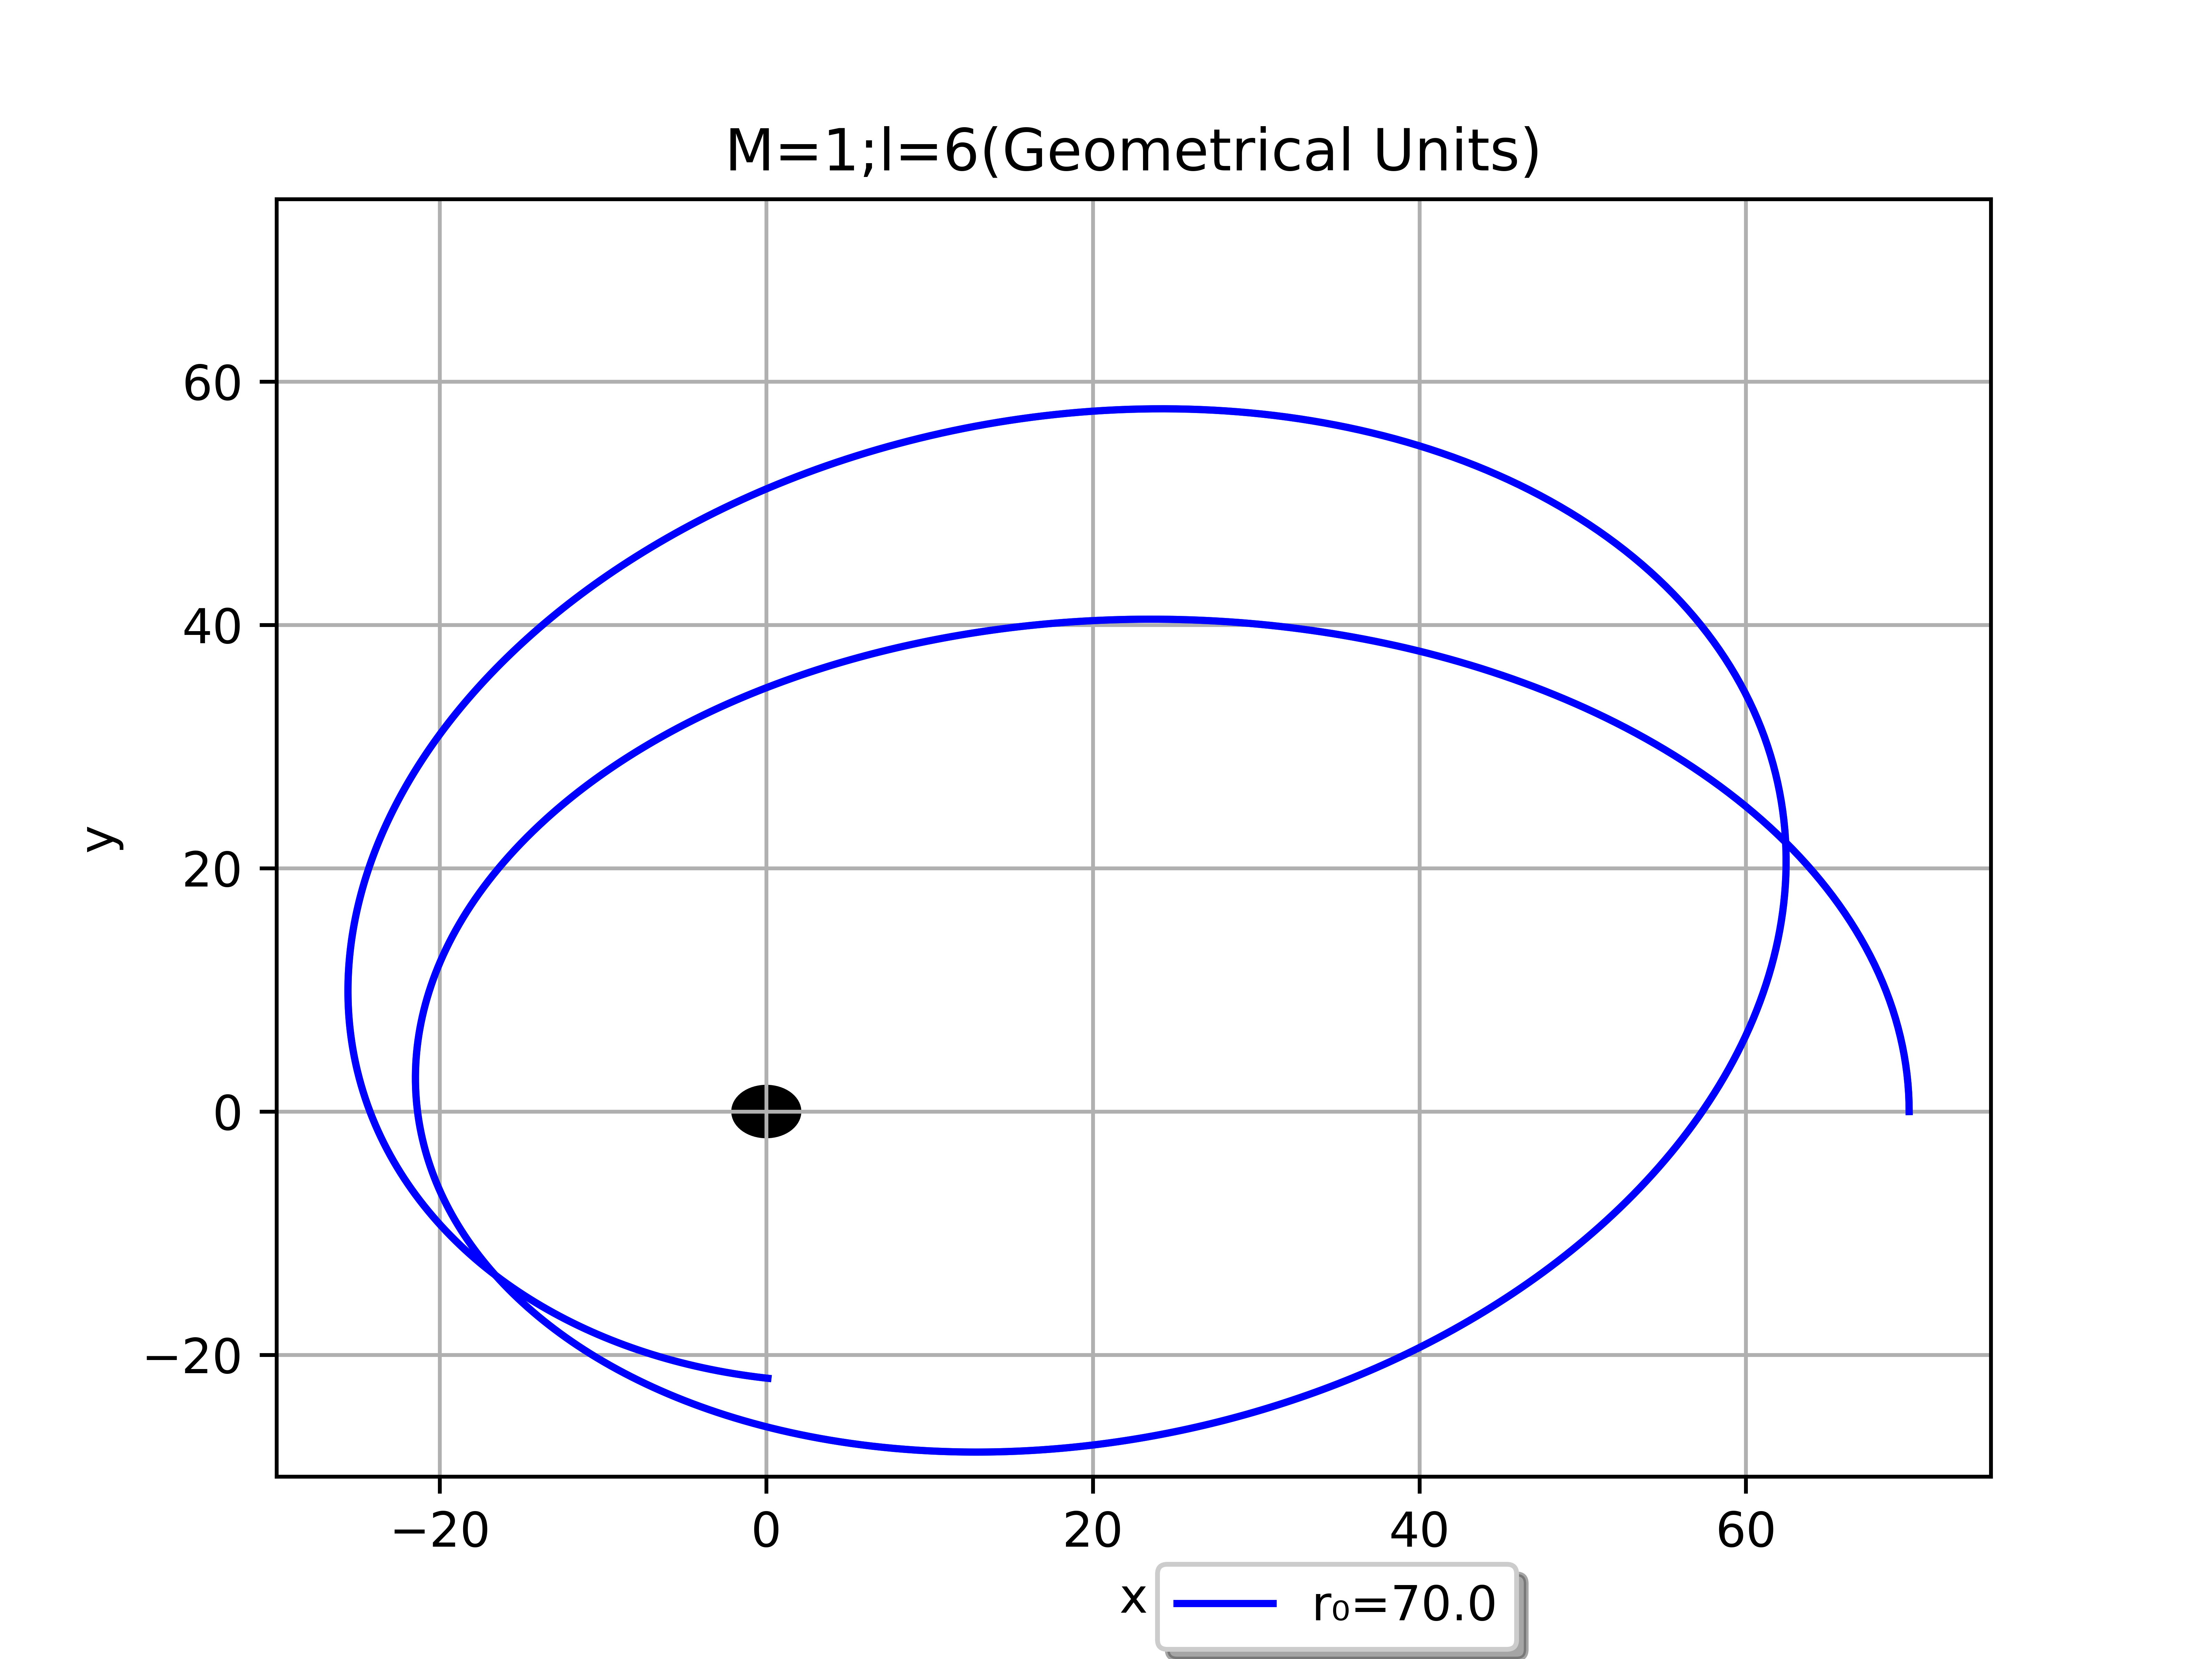
\includegraphics[width=0.9\linewidth, height=6cm]{SchwarzschildOrbit.png} 
\caption{Trayectoria de una partícula masiva en la métrica de Schwarzschild, fuente: elaboración propia.}
\label{fig:SchwarzschildOrbit}
\end{subfigure}\hspace{1cm}
\begin{subfigure}{0.5\textwidth}
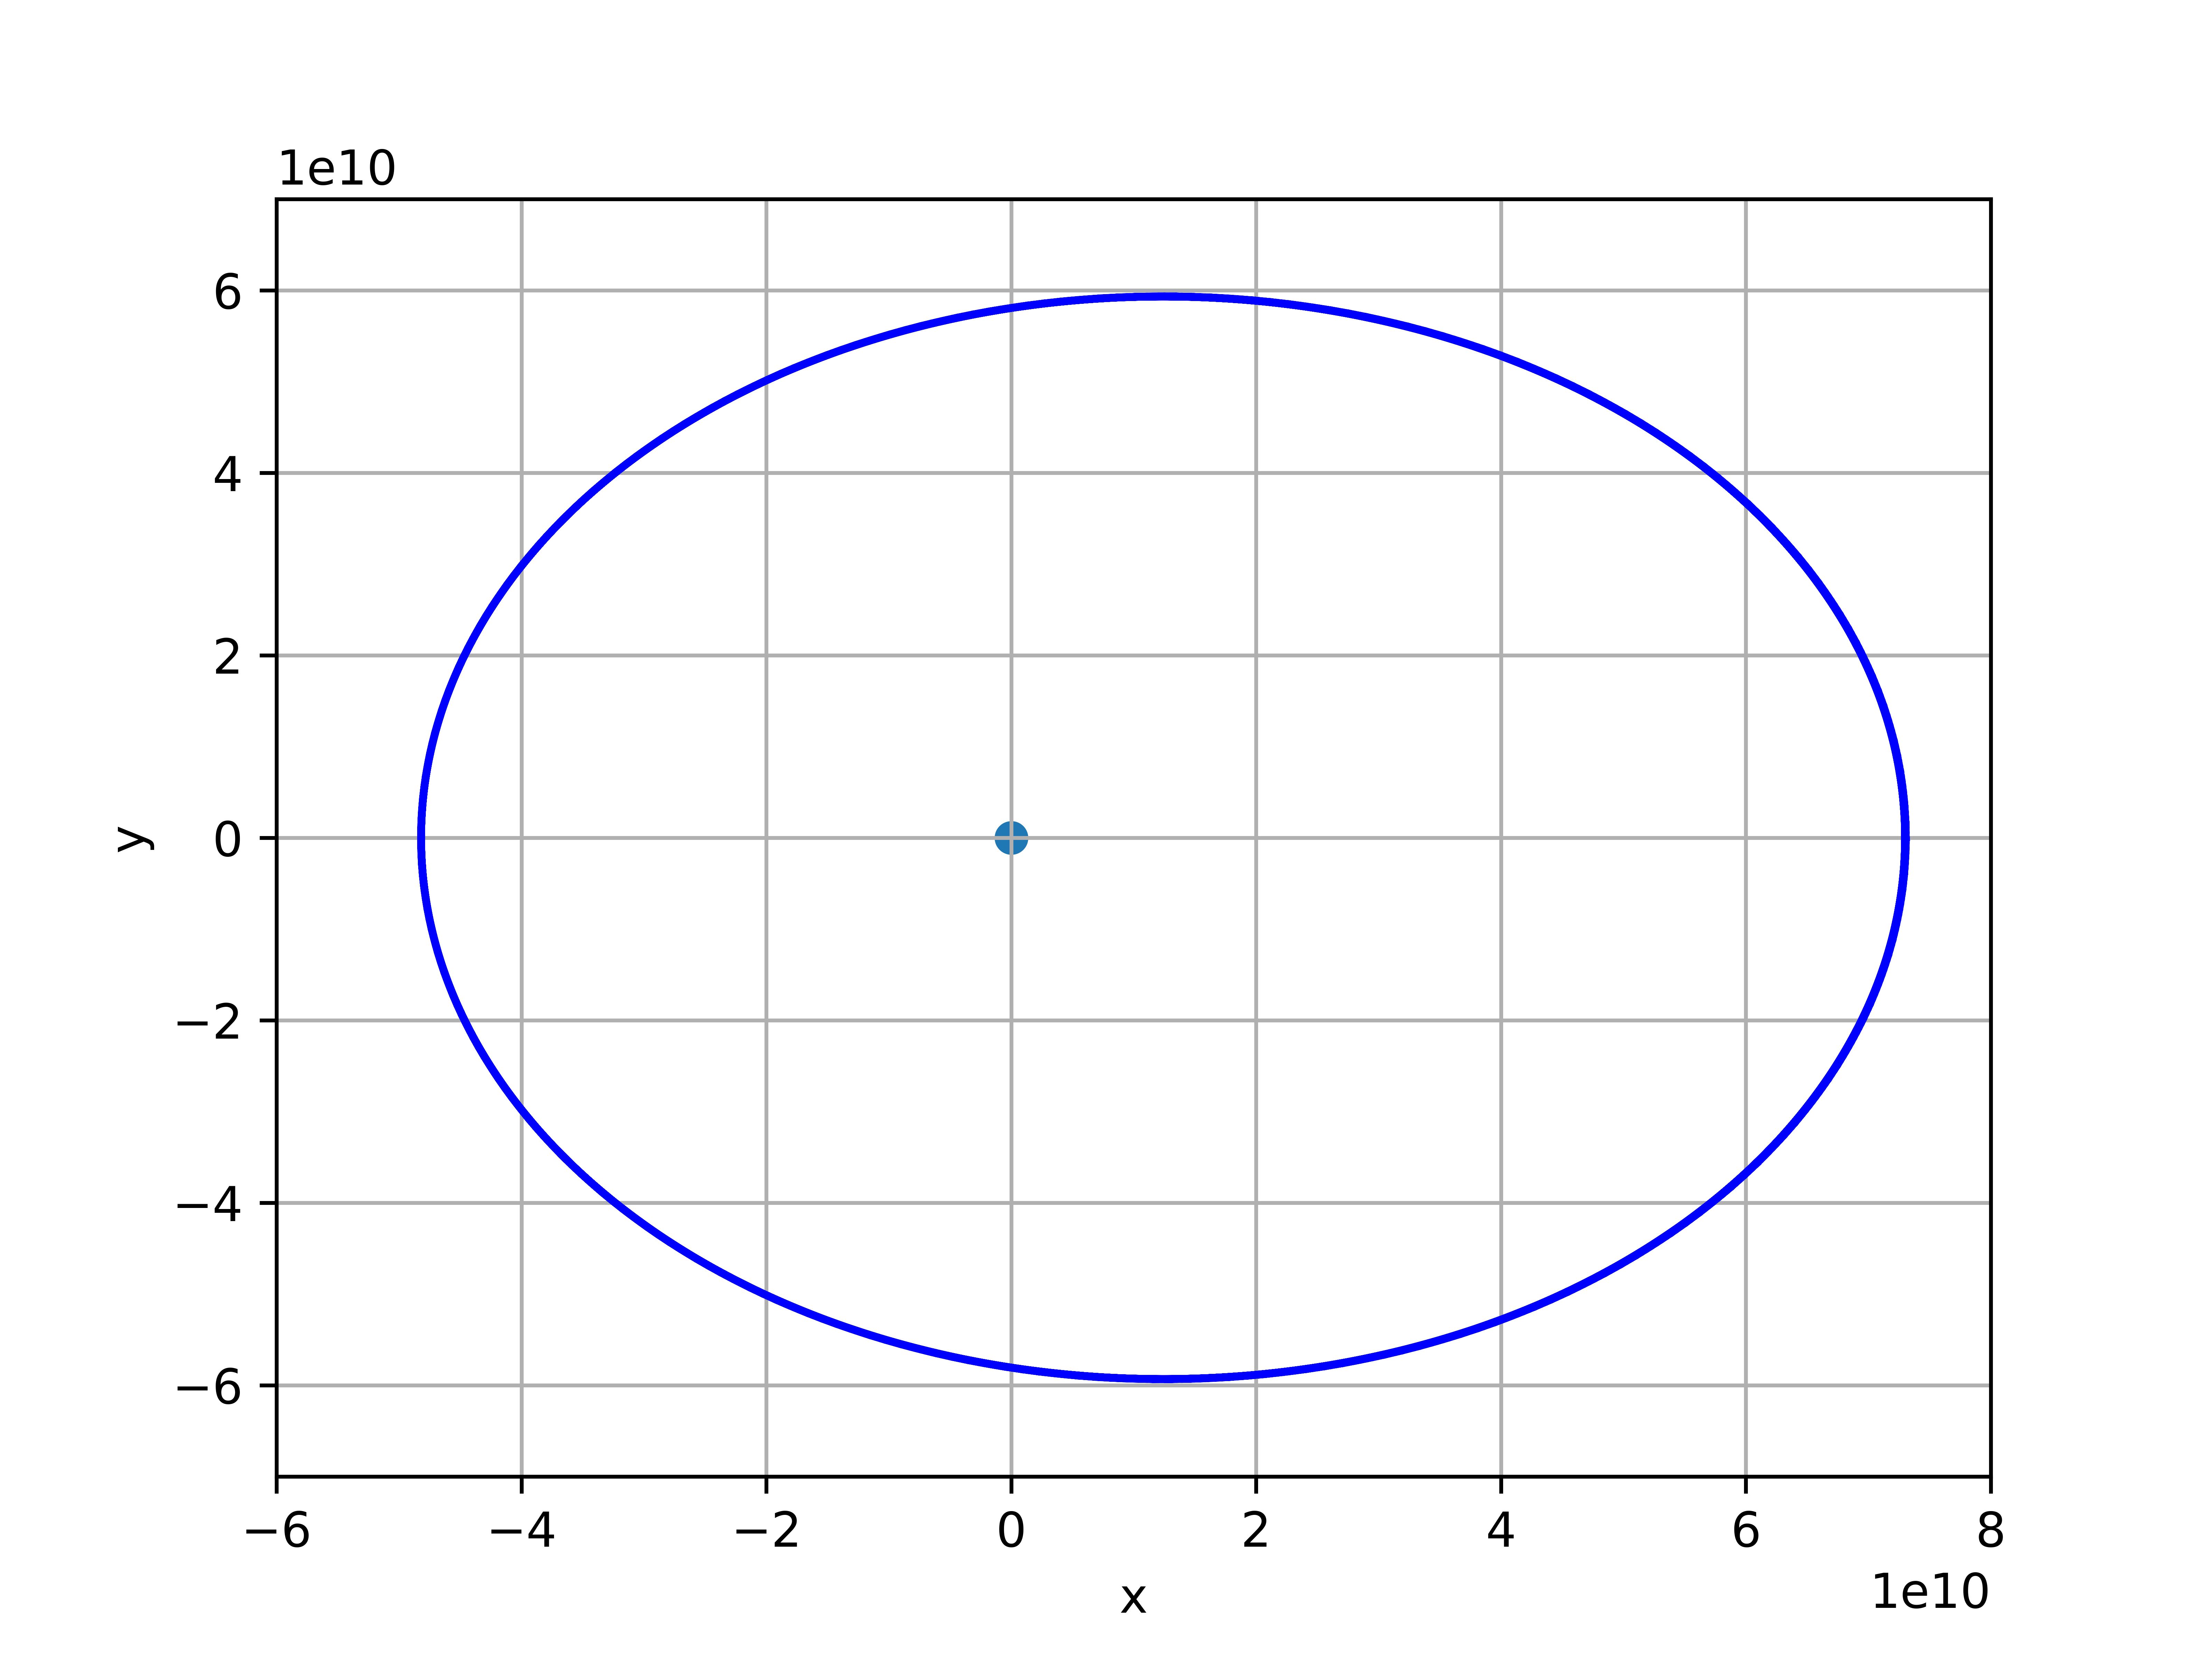
\includegraphics[width=0.9\linewidth, height=6cm]{ClassicOrbit.png}
\caption{Trayectoria de un planeta alrededor de una estrella según la mecánica Newtoniana; $M=1.98 10^{30}kg$, $m=3.285 10^{23}kg$, $l=9.1 10^{38}kg m^{2}/s$, $\epsilon=0.205$, fuente: elaboración propia.}
\label{fig:ClassicOrbit}
\end{subfigure}
\caption{Comparación del movimiento de una partícula en la métrica de Schwarzschild con la mecánica Newtoniana.}
\label{fig:image2}
\end{figure}

Se puede apreciar una precesión apsidal producido por la propia métrica (Fig: \ref{fig:SchwarzschildOrbit}), no como en la mecánica Newtoniana (Fig: \ref{fig:ClassicOrbit}), normalmente todos los planetas tienen una precesión debida entre otras cosas por la atracción de los otros planetas, pero aquí la propia métrica provoca este movimiento.

Para las trayectorias de los rayos de luz debemos usar las geodésicas nulas, es decir:\cite{zamorageodesicas}

\begin{equation}
    \mathcal{L}=g_{ij}\dot x^{i}\dot x^{j}=0
\end{equation}

En este caso obtenemos:\cite{zamorageodesicas}

\begin{align}\label{23}
    \frac{1}{b^{2}}=\frac{1}{l^{2}}\left(\frac{dr}{d\lambda}\right)^{2}+W_{efe}(r)
    && b^{2}=\frac{e^{2}}{l^{2}} && Wefe(r)=\frac{1}{r^{2}}\left(1-\frac{2M}{r}\right)
\end{align}

Como antes, haciendo el cambio $\frac{dr}{d\tau}=\frac{dr}{d\phi}\frac{d\phi}{d\tau}$, $r=1/u$ y derivando otra vez respecto de $\phi$, obtenemos:\cite{zamorageodesicas}

\begin{equation}
    \frac{d^{2}u}{d^{2}\phi}=3Mu^{2}-u
\end{equation}

Podemos analizar también esta ecuación mediante un Runge-Kutta de orden 4.

\begin{figure}[H]\label{S_light}
    \centering
    \includegraphics[width=0.9\textwidth]{Schwarszchild_Light.png}
    \caption{Trayectoria de la luz en la métrica de Schwarzschild para una masa M=1. En negro se representa un circulo de radio 2M que sería el agujero en si mismo, en rojo un circulo de radio 3M que corresponde a la fotoesfera y en azul la trayectoria de la luz, fuente: elaboración propia.}
    \label{fig:S_light}
\end{figure}
Podemos apreciar en (Fig: \ref{fig:S_light}) perfectamente como la trayectoria de la luz se curva al acercarse al agujero negro, es totalmente novedoso, porque si estuviéramos en la mecánica Newtoniana los fotones no se verían afectados por la gravedad al no tener masa.

Es interesante apreciar perfectamente la fotoesfera (en rojo), que es la ultima frontera para la luz, ya que si la cruzan los fotones, estos caen irremediablemente al agujero negro, por eso esta esfera es lo único que podremos ver nunca de un agujero negro. 

La fotoesfera viene ya caracterizada en las ecuaciones del movimiento, basta con buscar los máximos del potencial efectivo (\ref{23})\cite{zamorageodesicas}:

\begin{equation}
    \frac{dWefe}{dr}=-\frac{2}{r^{3}}+\frac{6M}{r^{4}}=0
\end{equation}

\begin{equation}
    r_{max}=3M
\end{equation}

\section{Agujeros negros en rotación}

Los agujeros negros de Schwarzschild son una buena aproximación teórica pero los agujeros negros reales suelen tener por lo que se sabe un momento angular no nulo.

Necesitamos de una métrica más sofisticada que describa el espacio-tiempo generado por objetos en rotación, mucho más apta para describir una enorme variedad de sistemas astrofísicos.\cite{jeffersonagujeros}\cite{kerr1963gravitational}

La solución de Kerr representa la única solución de vacío que la Teoría General de la Relatividad provee para describir a un agujero negro rotante estacionario y sin carga eléctrica. Esta solución es un caso particular de una solución a las ecuaciones de Einstein-Maxwell: la llamada métrica de Kerr-Newman que describe a un agujero negro rotante y con carga eléctrica. A pesar de esto, los agujeros de Kerr tienen mayor relevancia astrofísica ya que es de esperar que, por acreción de material, los agujeros negros cargados tiendan a neutralizarse rápidamente.\cite{sandoval2009perturbaciones}

\subsection{Métrica de Kerr}

Para obtener la solución de Kerr hay que hacer varias suposiciones; dado que el objeto se encuentra en constante rotación es razonable pensar que la
métrica buscada se caracterice no solo por el parámetro de masa M sino también por su momento angular J.\cite{jeffersonagujeros}

Para la descripción de dicho espacio-tiempo, es conveniente introducir la
coordenada temporaloide $t(= x_{0})$ y el ángulo azimutal $\phi( x_{3})$ para el eje de simetría. El carácter estacionario y con simetría axial del espacio-tiempo requiere que los coeficientes de la métrica $g( x_{\mu\nu})$ sean independientes de $t$ y $\phi$. Por lo tanto, los coeficientes dependerán a lo sumo de $r$ y $\theta$.\cite{jeffersonagujeros}

Además de la estacionalidad y la simetría axial, también requeriremos que el elemento de línea sea invariante para la inversión simultánea de las coordenadas $t$ y $\phi$, es decir, las transformaciones:\cite{jeffersonagujeros}

\begin{align*}
    t \xrightarrow[]{} -t && \phi \xrightarrow[]{} -\phi
\end{align*}

El significado físico de este requerimiento se encuentra ligado directamente a que la fuente de campo gravitacional se encuentra rotando alrededor de un eje de simetría, se deben considerar nulos los coeficientes:\cite{jeffersonagujeros}

\begin{equation}
    g_{01}=g_{10}=g_{02}=g_{20}=g_{13}=g_{31}=g_{13}=g_{23}=g_{32}=0
\end{equation}

La métrica toma esta forma:

\begin{equation}\label{15}
    ds^{2}=
    g_{00}dt^{2} 
    +2g_{03}dtd\phi 
    +g_{33}d\phi^{2}
    +\left[g_{11}(dx^{1})^{2}+2g_{12}dx^{1}dx^{2}+g_{22}(dx^{2})^{2}
    \right]
\end{equation}


Observamos que, dado que los coeficientes métricos $g_{\mu\nu}$ son funciones solo de $x_{1}$ y $x_{2}$, la expresión entre corchetes en se puede considerar como un submanifold 2-dimensional.\cite{jeffersonagujeros}

Por lo tanto, se puede lograr una reducción adicional en la forma de la métrica utilizando el hecho de que cualquier variedad pseudoriemanniana 2-dimensional es conformacionalmente plana, es decir, siempre es posible encontrar un sistema de coordenadas en el que la métrica adopte la forma; $g_{ab}=\Omega^{2}(x)\eta_{ab}$. Donde $\Omega^{2}(x)$ es una función arbitraria de las coordenadas y $[\eta_{ab}] = diag(\pm1, \pm1)$, los signos dependen de la signatura de la variedad. Por lo tanto, aprovechando este hecho, y escribiendo el resultado para un cuerpo en rotación, podemos expresar el elemento de línea (\ref{15}) en la forma:\cite{jeffersonagujeros}

\begin{equation}\label{16}
    ds^{2}=
    Adt^{2} 
    -B(dtd\phi -\omega dt)
    -Cdr^{2}
    -Dd\theta^{2}
\end{equation}

Donde A, B, C, D y $\omega$ son funciones arbitrarias de las coordenadas espacialoides $r$ y $\theta$, pero tenemos la libertad de relacionar C y D de tal manera que los significados físicos
de $r$ y $\theta$ estén lo más cerca posible al caso de coordenadas esféricas convencionales. Las funciones (\ref{16}) están relacionados con los coeficientes métricos $g_{\mu\nu}$ por:\cite{jeffersonagujeros}

\begin{align*}
   g_{tt}=A-B\omega^{2} && g_{t\phi}=B\omega && g_{\phi\phi}=-B && g_{rr}=-C && g_{\theta\theta}=-D
\end{align*}

Para obtener la solución de Kerr, basta con de imponer estacionariedad y simetría axial, en contraposición con la estaticidad y simetría esférica de Schwarzschild. Se trata, igual que esta, de una solución para el vacío $(T_{\mu\nu} = 0$).\cite{jeffersonagujeros} 

\begin{equation}\label{Kerr}
    ds^{2}=
    -\left(1-\frac{2GMr}{c^{2}\Sigma}\right)c^{2}dt^{2} 
    -\frac{4aGMrsen^{2}\theta}{c^{3}\Sigma}cdtd\phi 
    +\frac{\Sigma}{\Delta}dr^{2}
    +\Sigma d\theta^{2} 
    +\left(r^{2}+\frac{a^{2}}{c^{2}}+\frac{2a^{2}Mrsen^{2}\theta}{c^{4}\Sigma}\right)sen^{2}\theta d\phi^{2}
\end{equation}
donde;
\begin{align}
  \Sigma=r^{2}+\frac{a^{2}}{c^{2}}cos^{2}\theta  && \Delta=r^{2}-\frac{2GMr}{c^{2}}+\frac{a^{2}}{c^{2}}
\end{align}

En ella, M y a son constantes de integración que caracterizan nuestro sistema. La constante a es llamada parámetro de Kerr y se define como $a=J/M$ es su momento angular por unidad de masa. La métrica de Kerr tiene las siguientes características:\cite{jeffersonagujeros} 

\begin{enumerate}
    \item Es estacionaria, la métrica no depende explícitamente del tiempo.
    \item Tiene simetría axial, la métrica no depende explícitamente de la coordenada $\phi$.
    \item La métrica no es estática. No es invariante ante transformaciones de reversión $t \xrightarrow[]{} -t$ temporal.
    \item La métrica es invariante ante transformaciones simultáneas de reversión en el tiempo $t \xrightarrow[]{} -t$ y reversión en la coordenada angular $\phi \xrightarrow[]{} -\phi$.
    \item En el límite $r \xrightarrow[]{} \infty$, la métrica de Kerr se reduce a la métrica de Minkowski.
    \item En el límite $a \xrightarrow[]{} 0$ y con $(M \neq 0)$, la métrica de Kerr se reduce a la métrica de Schwarzschild.
\end{enumerate}

\subsection{Horizonte de sucesos}

Un horizonte de eventos se define como una región causalmente desconectada del resto de universo. Es decir que las partículas que la atraviesen de un sentido no podrán hacerlo en el sentido contrario.\cite{borghiagujeros}

En su interior, ni siquiera partículas sin masa (fotones) pueden escapar, y cualquier fotón emitido justo sobre esta superficie se mantendrá en movimiento estacionario sobre ella.
Se tiene por tanto que cualquier observador que viaje mas allá del horizonte de sucesos perderá completamente su capacidad de influir al exterior, se habrá roto el contacto causal.\cite{jeffersonagujeros}

Si estudiamos la métrica de Kerr observaremos que esta diverge en $\Delta$=0, esta singularidad define dos superficies tal que: \cite{borghiagujeros}

\begin{equation}
    r_{\pm}=M \pm \sqrt{M^{2}-a^{2}}
\end{equation}

Esto define dos regiones. La exterior r+ es el horizonte de eventos del agujero negro. Mientras que r- define una superficie que se llama el horizonte de Cauchy.\cite{borghiagujeros}Ambos tienen forma elipsoidal, podemos ver que existen diferentes soluciones dependiendo de la relación entre a y M.\cite{jeffersonagujeros}

\begin{enumerate}
    \item Caso subextremal: $a < M$. Existen dos horizontes de sucesos bien diferenciados.
    Para $r_{-} < r < r_{+}$, no existe ningún vector de Killing de tipo temporal y por lo tanto es imposible llevar una trayectoria estacionaria: cualquier partícula que atraviese el primer horizonte se vera obligada a avanzar inexorablemente hasta alcanzar el segundo horizonte, momento en el cual la estacionariedad vuelve a ser posible.\cite{jeffersonagujeros}
    \item Caso extremal: $a = M$. La ecuación tiene una raiz doble en $r = M$. Este caso es un límite teórico poco realista. Ambos horizontes quedarían superpuestos, de modo que es imposible para un sistema con masa permanecer estacionario sobre la superficie, pero es perfectamente posible a cualquier lado de esta.\cite{jeffersonagujeros}
    \item Caso sobreextremal: $a > M$. No existen soluciones reales para $r$, de modo que no hay horizonte de sucesos y la singularidad queda desnuda. Los espacios con singularidades desnudas son altamente patológicos, debido a que la singularidad es capaz de influenciar causalmente y de forma incontrolada a cualquier punto del espacio-tiempo.\cite{jeffersonagujeros}
\end{enumerate}

Si $g_{tt}=0$, esto define una región de suma importancia llamada superficie límite estacionaria, donde, por ejemplo, una partícula masiva que incida sobre la misma independientemente de la velocidad con que incida empezar´a a moverse en la misma dirección que el agujero negro rotante.\cite{borghiagujeros}

\begin{equation}
    g_{tt}=0=1-\frac{2Mr}{r^{2}+a^{2}cos^2\theta}
\end{equation}
Esta condición nos lleva a una ecuación de segundo grado que tiene por tanto dos soluciones para r:
\begin{equation}
    s_{\pm}=M \pm \sqrt{M^{2}-a^{2}cos^{2}\theta}
\end{equation}

\begin{figure}[H]
    \centering
    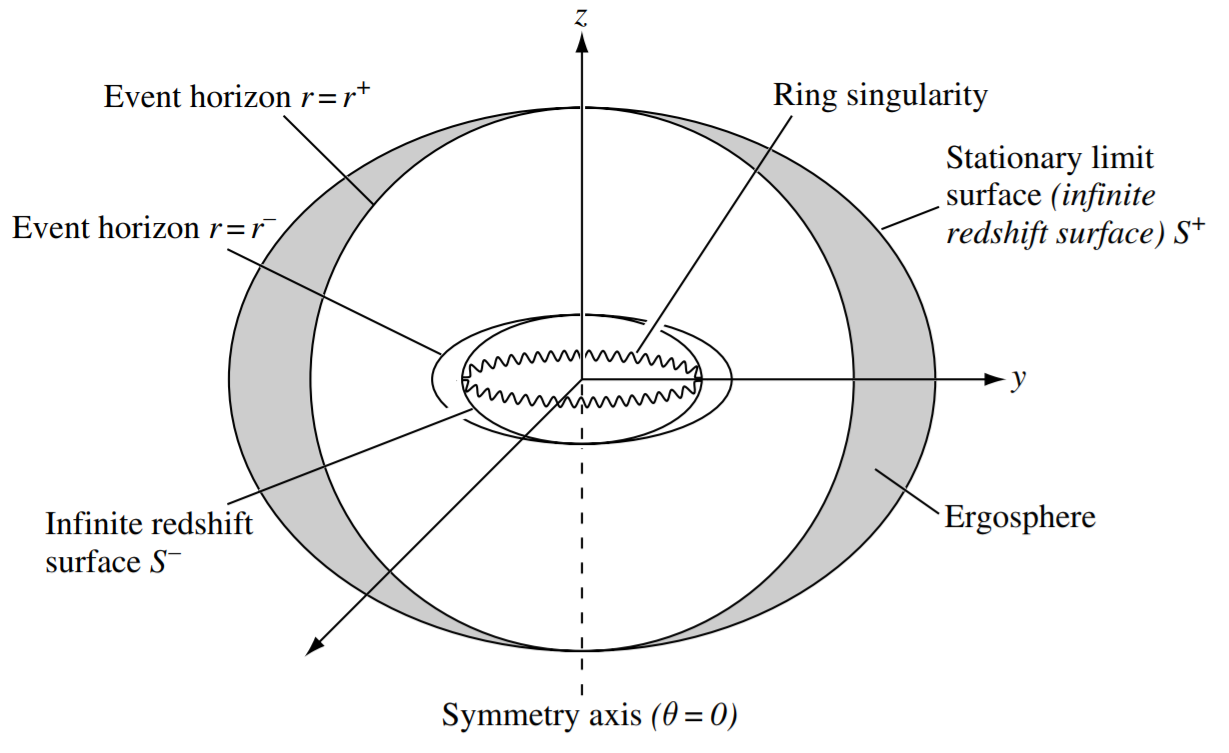
\includegraphics[width=0.7\textwidth]{Esquema_ANKerr_Jefferson.png}
    \caption{Esquema de un Agujero Negro de Kerr, fuente: \cite{jeffersonagujeros}}
    \label{fig:Esquema_ANKerr}
\end{figure}

Se puede apreciar en (Fig: \ref{fig:Esquema_ANKerr}), las distintas capas del agujero negro.

\subsection{Geodésicas en la métrica de Kerr}

Las orbitas en la métrica de Kerr no estan confinadas en ningún plano porque la magnitud que se conserva es la componente del momento angular paralela al eje de simetría, salvo en el plano ecuatorial que si lo son $\theta=\pi/2$. La métrica quedaría:\cite{zamorageodesicas}

\begin{equation}\label{Kerr}
    ds^{2}=
    -\left(1-\frac{2Mr}{\rho^{2}}\right)dt^{2} 
    -\frac{4aM}{r}dtd\phi 
    +\frac{r^{2}}{\Delta}dr^{2}
    +\Sigma d\theta^{2} 
    +\left(r^{2}+a^{2}+\frac{2Ma^{2}}{r}\right) d\phi^{2}
\end{equation}

En este caso las ecuaciones de las trayectorias para las partículas quedan como:

\begin{align}
    \frac{dt}{d\tau}=\frac{1}{\Delta}\left[\left(r^{2}+a^{2}+\frac{2Ma^{2}}{r}\right)e-\frac{2Ma}{r}l\right]; && \frac{d\phi}{d\tau}=\frac{1}{\Delta}\left[\left(1-\frac{2M}{r}l\right)+\frac{2Ma}{r}e\right]
\end{align}

\begin{align}
    \mathcal{E}=\frac{e^{2}-1}{2}; && \frac{e^{2}-1}{2}=\frac{1}{2}\left(\frac{dr}{d\tau}\right)^{2}+V_{efe}(r,e,l)
\end{align}
El potencial efectivo sería:
\begin{equation}\label{39}
    V_{efe}(r,e,l)=\frac{-M}{r}+\frac{l^{2}-a^{2}(e^{2}-1)}{2r^{2}}-\frac{M(l-ae)^{2}}{r^{3}}
\end{equation}

La ecuación de las orbitas en el plano ecuatorial  quedaría de la forma $u(u=1/r)$ respecto de $\phi$: \cite{bambhaniya2021precession}

\begin{equation}\label{Kerr_Motion}
    \frac{d^{2}u}{d\phi^{2}}=\frac{1-2Mu+a^{2}u^{2}}{(l-2Mu(l-ae))^{3}}[M(l-2ae(e^{2}-1))+u(l(-l^{2}+3a^{2}(e^{2}-1))-2M^{2}(2l+2ae)+uB(u))]
\end{equation}
Donde:
\begin{multline*}
    B(u)=M(7l^{3}-6ael^{2}+a^{2}l(11-3e^{2})+2a^{3}e(e^{2}-1))+4M^{3}(l-ae)\\
    +u[-3a^{2}l^{3}+3a^{4}l(e^{2}-1)+2M^{2}(l-ae)(-8l^{2}+a(7le+a(e^{2}-5)))\\
    -Mu(l-ae)(a^{2}(-11l^{2}+a(7le+4a(e^{2}-1)))-12M^{2}(l-ae)^{2}+10a^{2}Mu(l-ae)^{2})]
\end{multline*}

Podemos por tanto representar haciendo un Runge-Kutta de orden 4 las trayectorias de las partículas alrededor de un agujero negro de Kerr.

\begin{figure}[H]
\begin{subfigure}{0.5\textwidth}
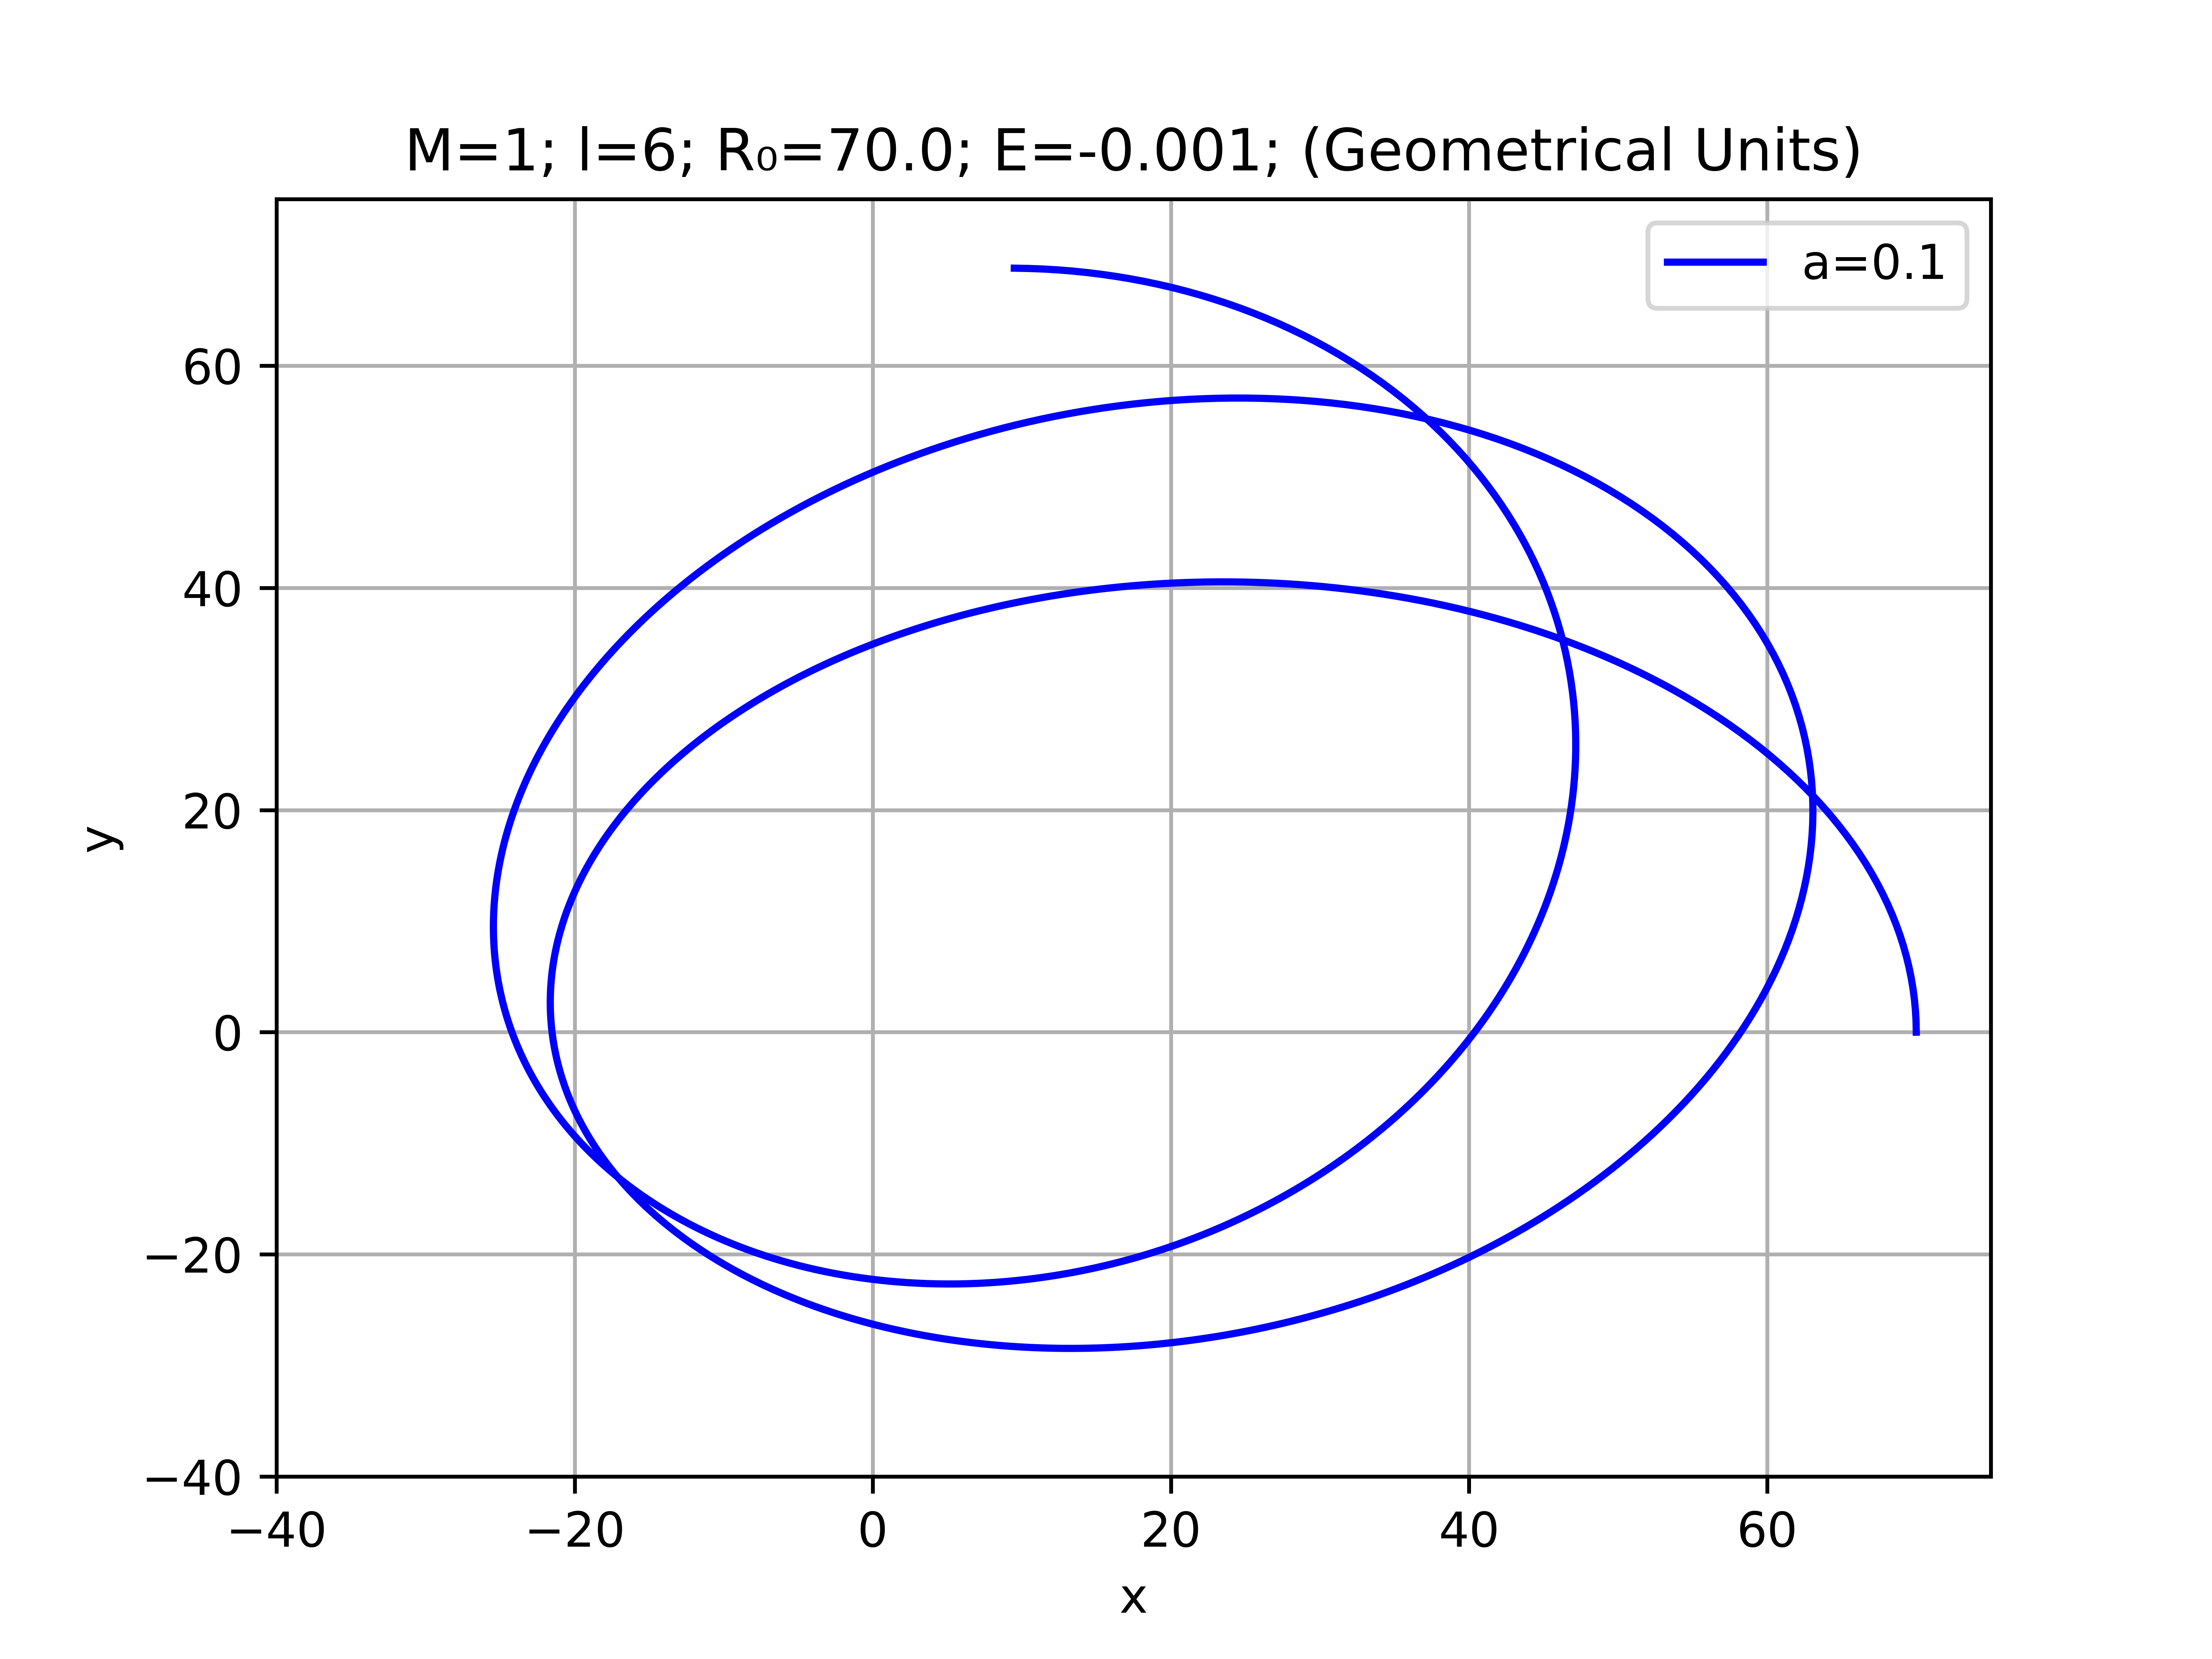
\includegraphics[width=0.9\linewidth, height=6cm]{KerrOrbit01.png} 
\caption{Trayectoria de una partícula para un agujero negro de momento angular $a=0.1$, fuente: elaboración propia.}
\label{fig:Kerr_orbit1}
\end{subfigure}\hspace{1cm}
\begin{subfigure}{0.5\textwidth}
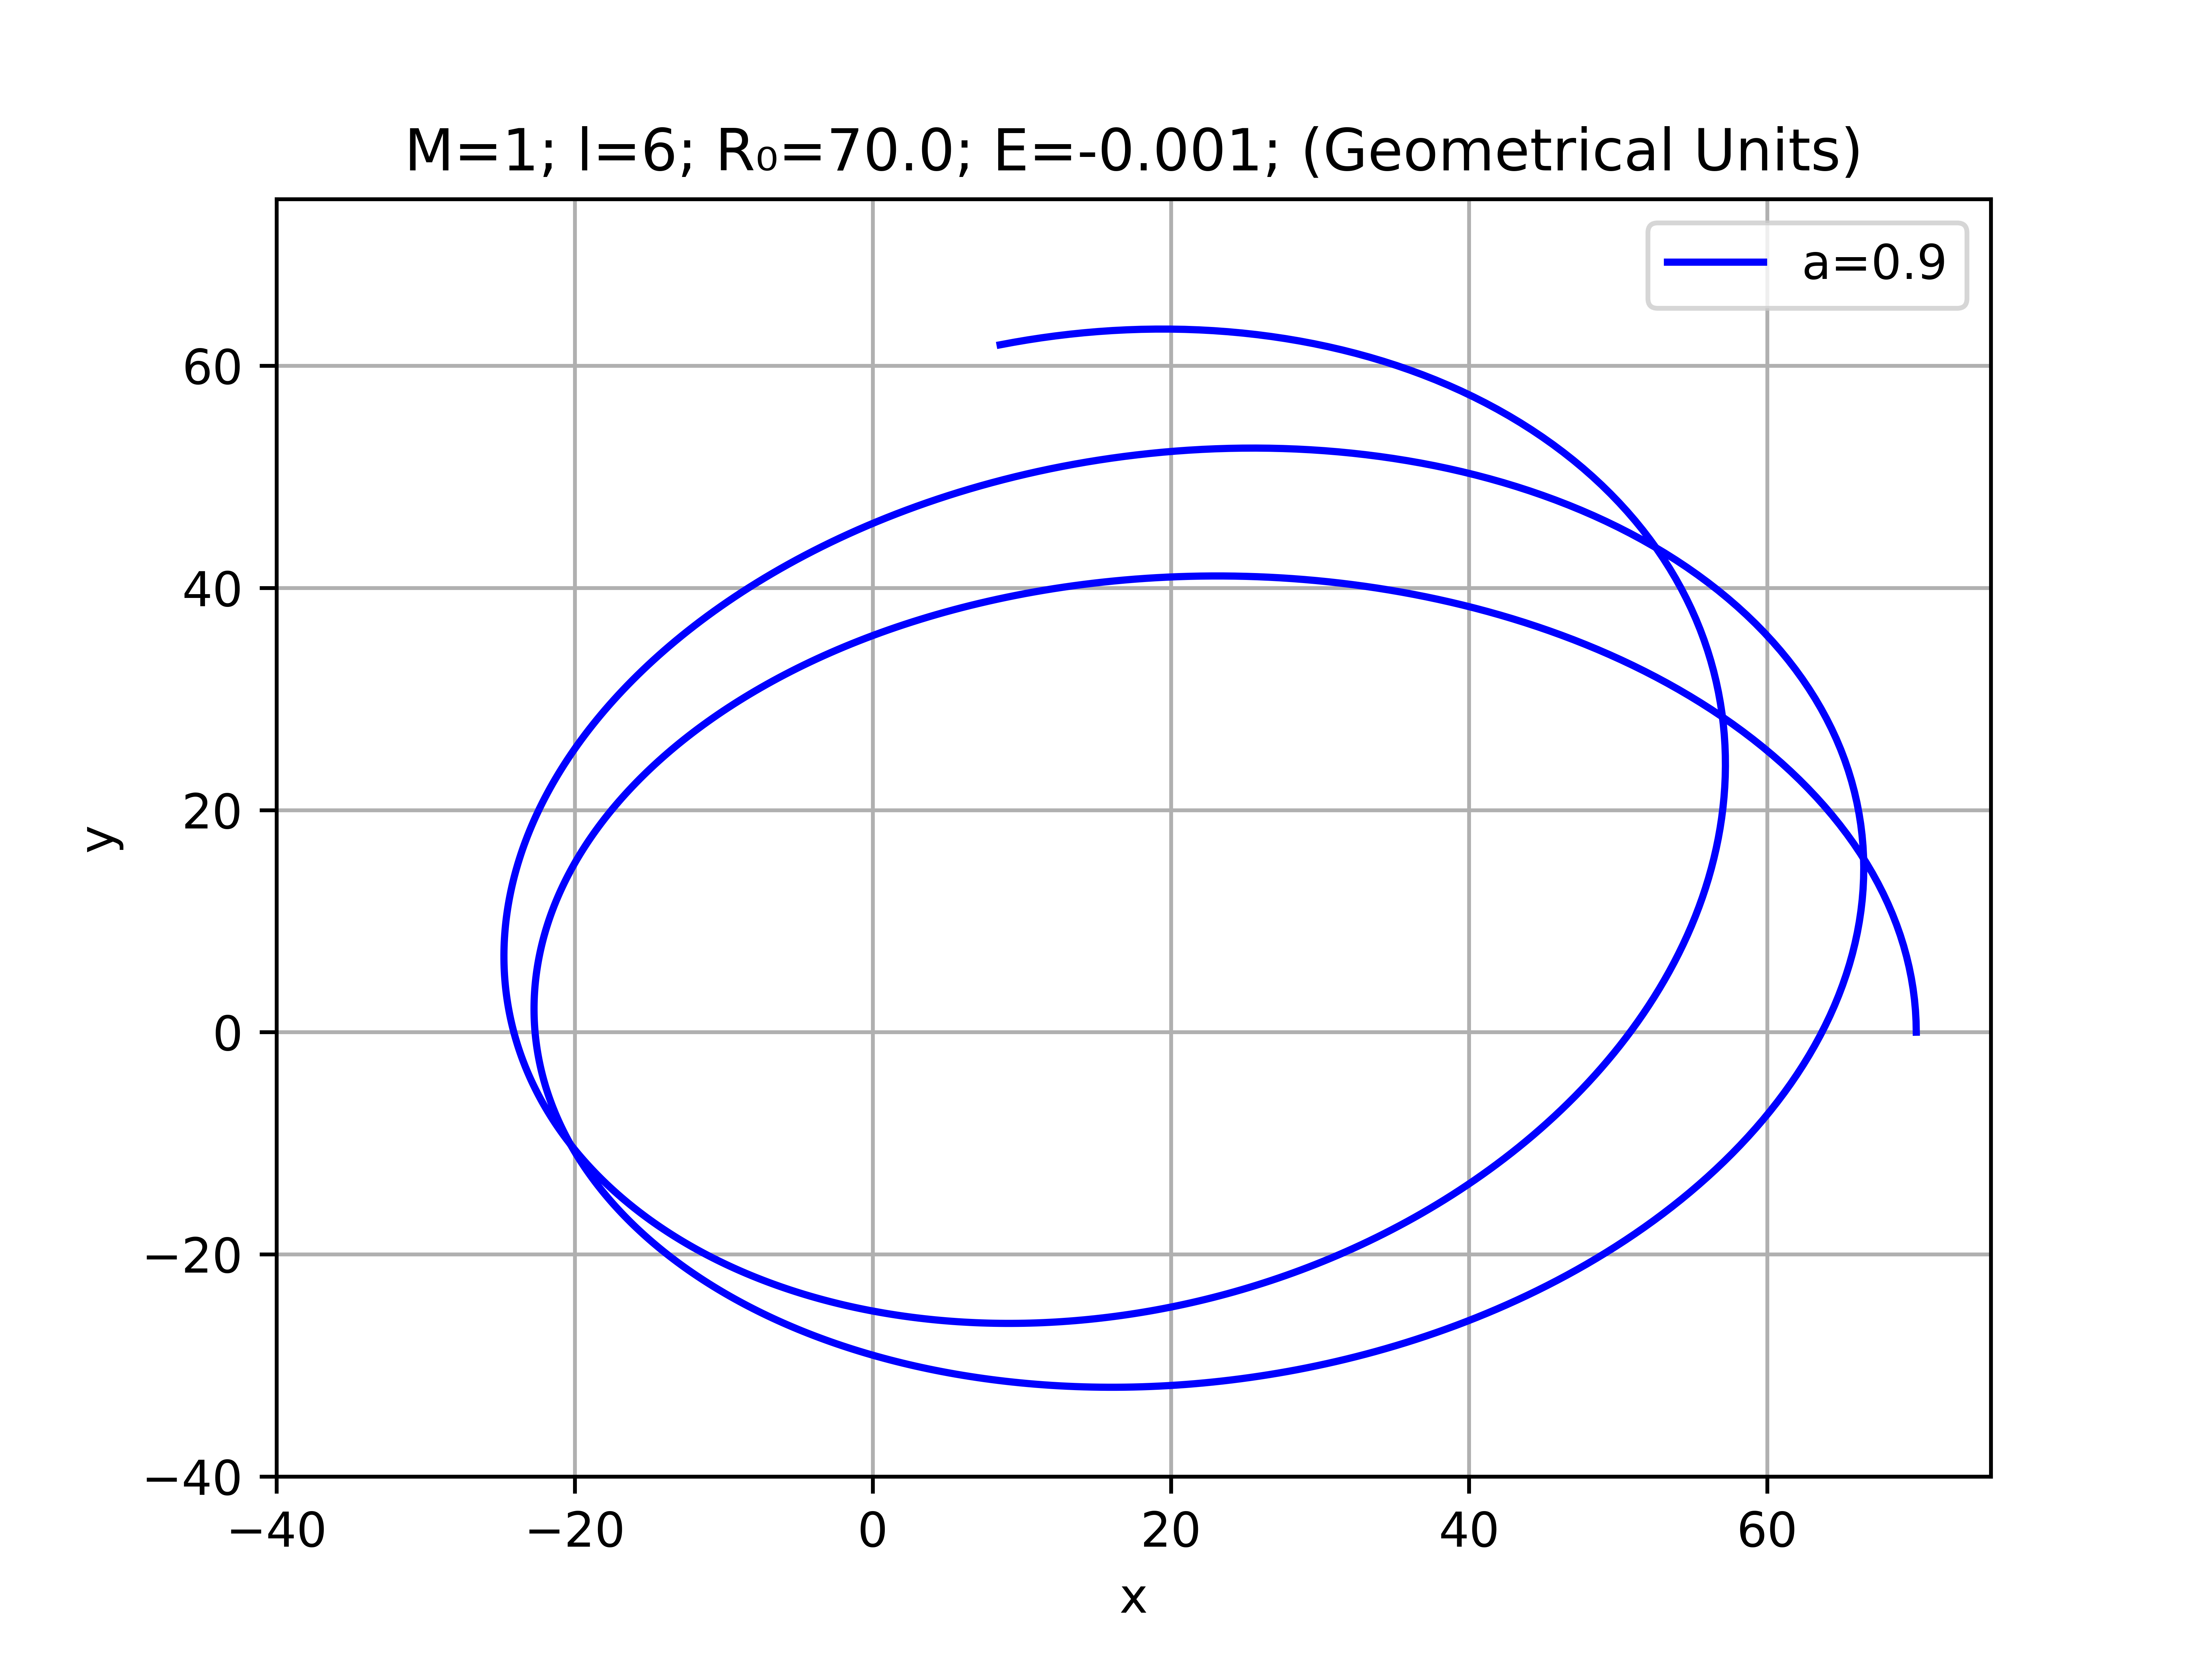
\includegraphics[width=0.9\linewidth, height=6cm]{KerrOrbit09.png}
\caption{Trayectoria de una partícula para un agujero negro de momento angular $a=0.9$, fuente: elaboración propia.}
\label{fig:Kerr_orbit2}
\end{subfigure}
\caption{Trayectoria de una partícula en la métrica de Kerr.}
\label{fig:Kerr_orbit}
\end{figure}

Con esta ecuación (\ref{Kerr_Motion}) podemos ver el movimiento de cualquier particula para cualquier valor de $a$, como en (Fig: \ref{fig:Kerr_orbit1}) y en (Fig: \ref{fig:Kerr_orbit2}).

Para la trayectoria de la luz nos quedan las ecuaciones del movimiento:\cite{zamorageodesicas}
\begin{equation}
    \frac{1}{l^{2}}\left(\frac{dr}{d\lambda}\right)^{2}=\frac{1}{b^{2}}-W_{efe}(r,b,\sigma)
\end{equation}
\begin{equation}
    W_{efe}(r,b,\sigma)=\frac{1}{r^{2}}\left[1-\left(\frac{a}{b}\right)^{2}-\frac{2M}{r}\left(1-\sigma\frac{a}{b}\right)^{2}\right]
\end{equation}

\begin{align}
  b= \abs[\Big]{\frac{l}{e}}  && \sigma=sign(l)
\end{align}

Podemos hacer un Runge-Kutta de orden 4 para representar la trayectoria de la luz en la métrica de Kerr como se puede ver en (Fig: \ref{fig:Kerr_Light}).

\begin{figure}[H]
    \centering
    \includegraphics[width=0.9\linewidth]{Kerr_Light.png}
    \caption{Trayectoria de la luz en la métrica de Kerr, fuente: elaboración propia.}
    \label{fig:Kerr_Light}
\end{figure}

\subsection{Innermost Spherical Circular Orbit (ISCO)}
El radio ISCO es el radio de la órbita circular estable más interno para una partícula,\cite{levin2008periodic} estas orbitas ocurren cuando el potencial V(r) alcanza un mínimo.\cite{misner1973gravitation}

Para el potencial efectivo para una partícula en la métrica de Schwarzschild:

\begin{equation}\cite{zamorageodesicas}
    V(r)=\frac{-M}{r}+\frac{l^{2}}{2r^{2}}-\frac{Ml^{2}}{r^{3}}
\end{equation}

Si buscamos los mínimos:

\begin{equation}\cite{zamorageodesicas}
    \frac{dV}{dr}=\frac{M}{r^{2}}-\frac{l^{2}}{r^{3}}+\frac{3Ml^{2}}{r^{4}}=0
\end{equation}

Si resolvemos la ecuación obtenemos dos soluciones, $R_{+}$ y $R_{-}$:

\begin{equation}
    R_{\pm}=\frac{l^{2}}{2M}\left(1\pm \sqrt{1-\frac{12M^{2}}{l^{2}}}\right)
\end{equation}

Podemos comprobar usando simulaciones que en estos dos radios obtenemos una orbita estable circular.

\begin{figure}[H]
\begin{subfigure}{0.5\textwidth}
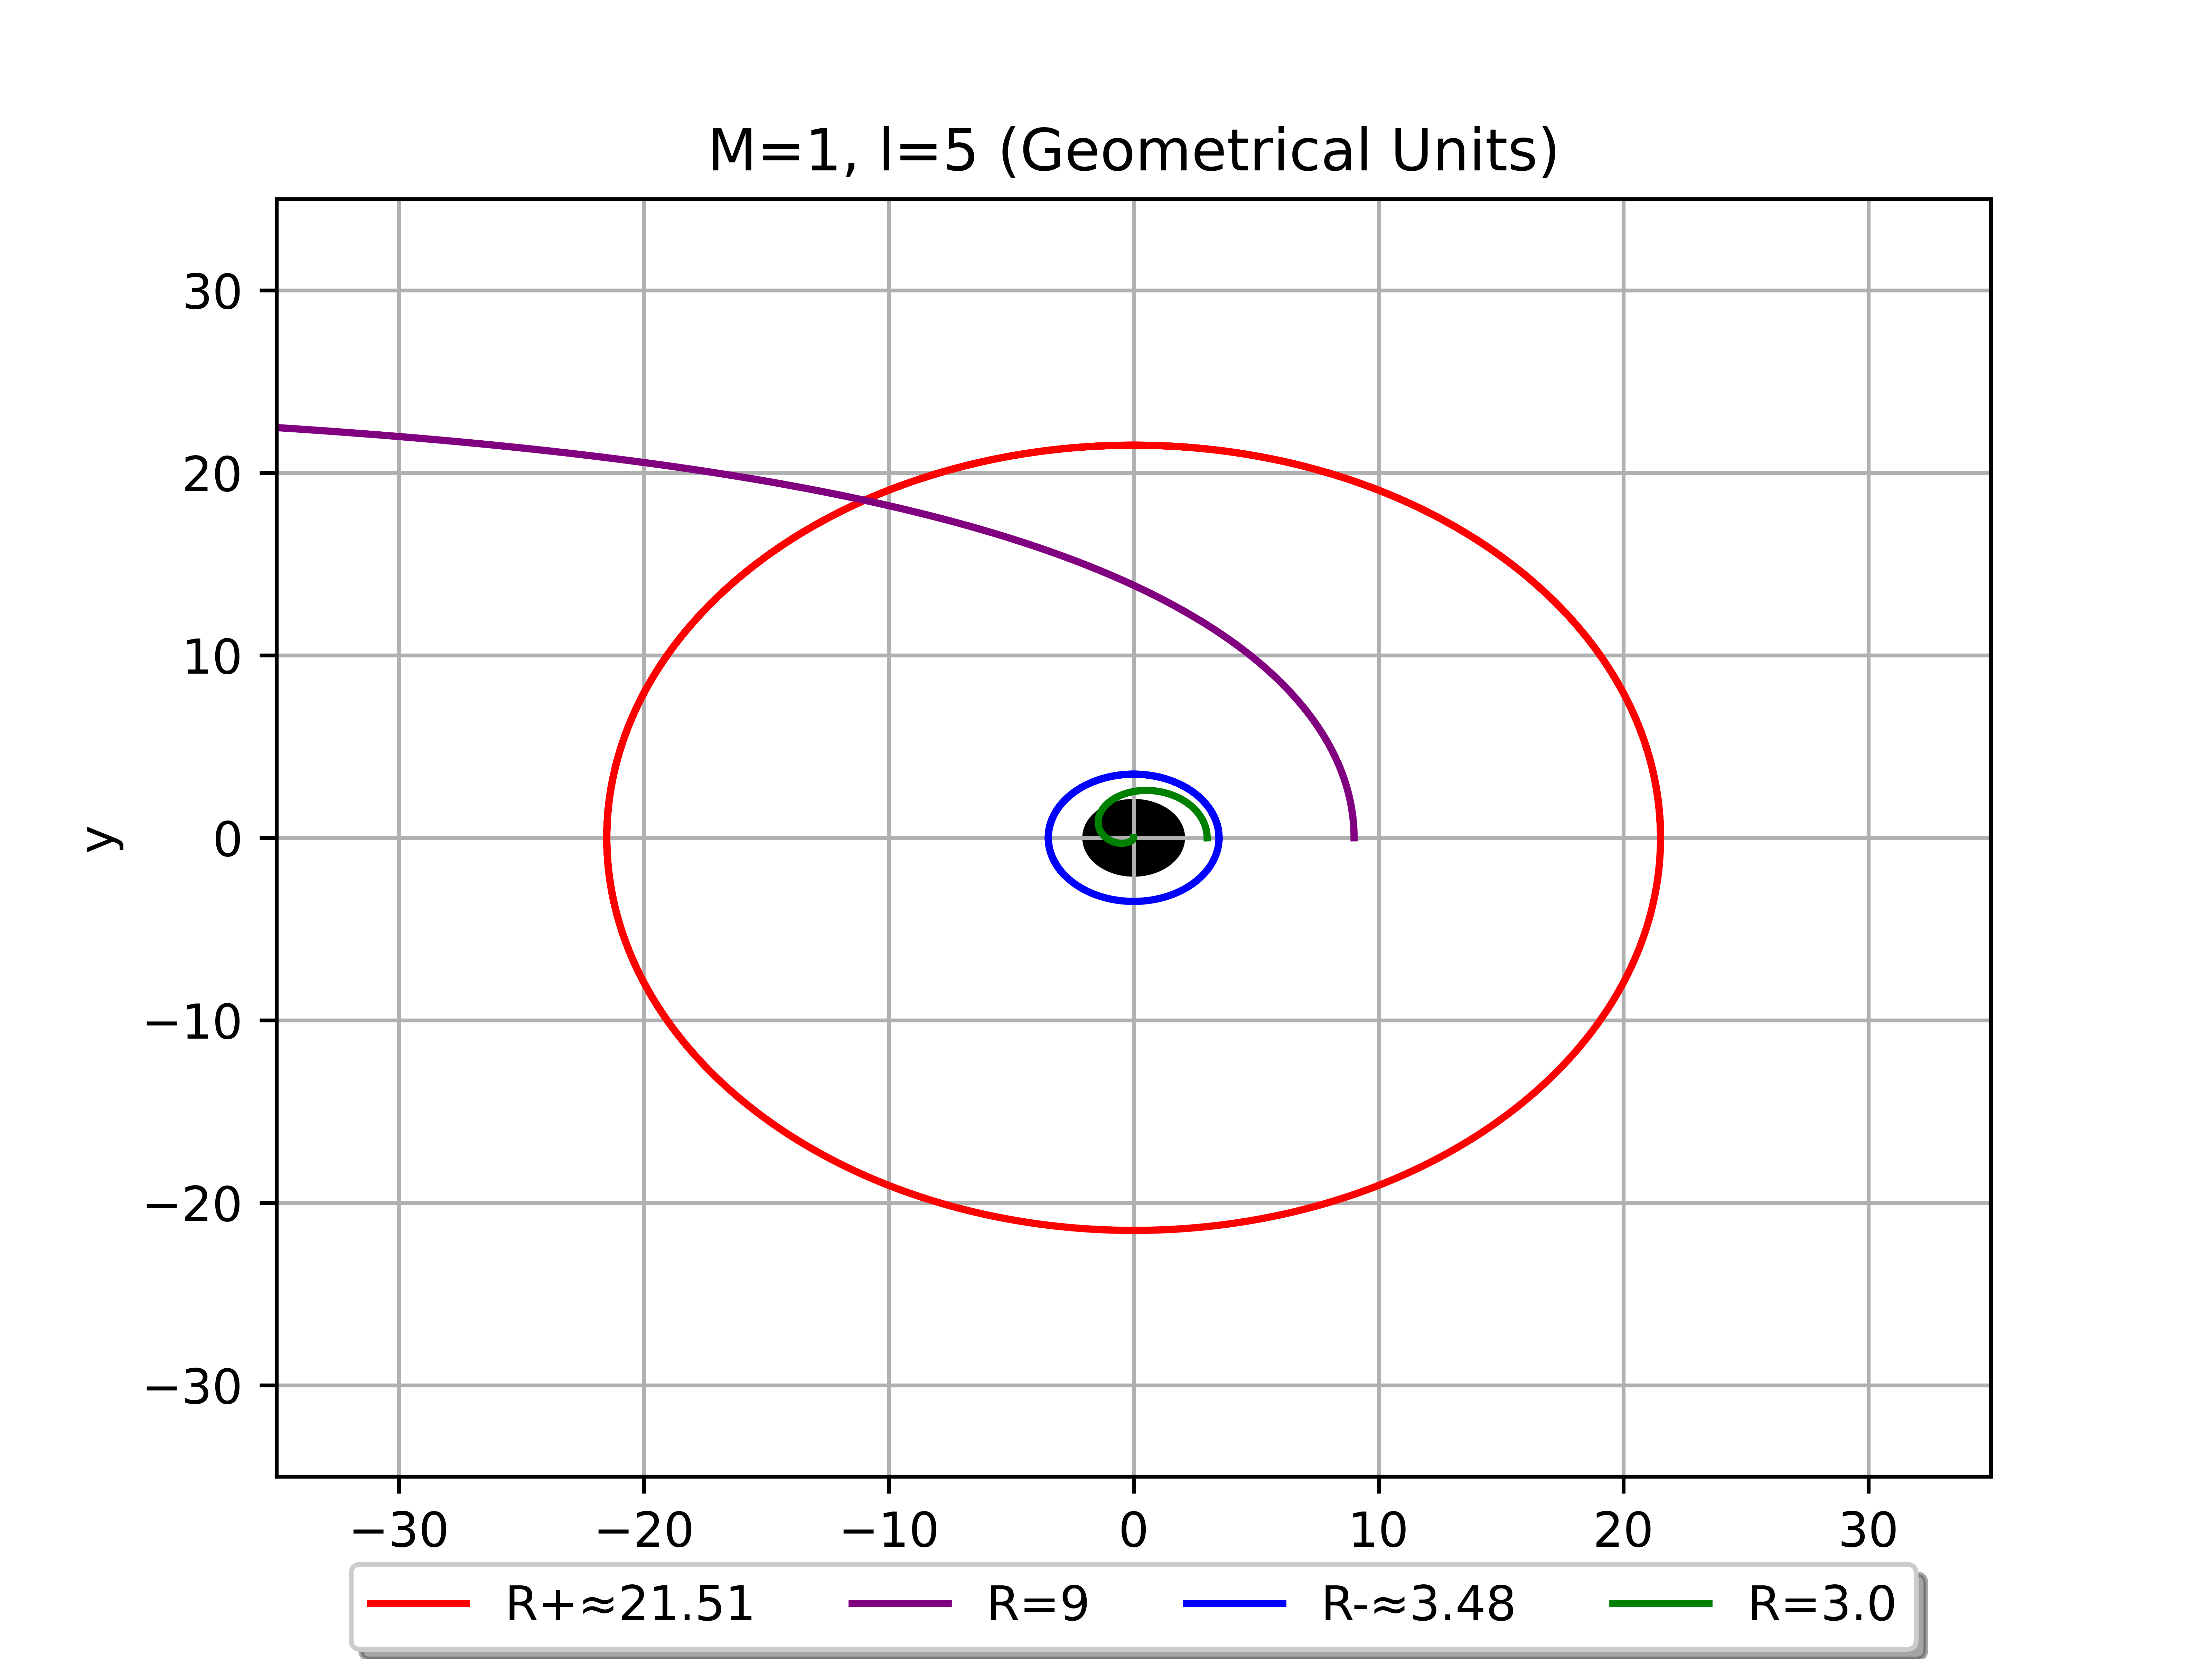
\includegraphics[width=0.9\linewidth, height=6cm]{ISCO.png} 
\caption{ISCO comparadas con orbitas inestables, fuente: elaboración propia.}
\label{fig:ISCO_S1}
\end{subfigure}\hspace{1cm}
\begin{subfigure}{0.5\textwidth}
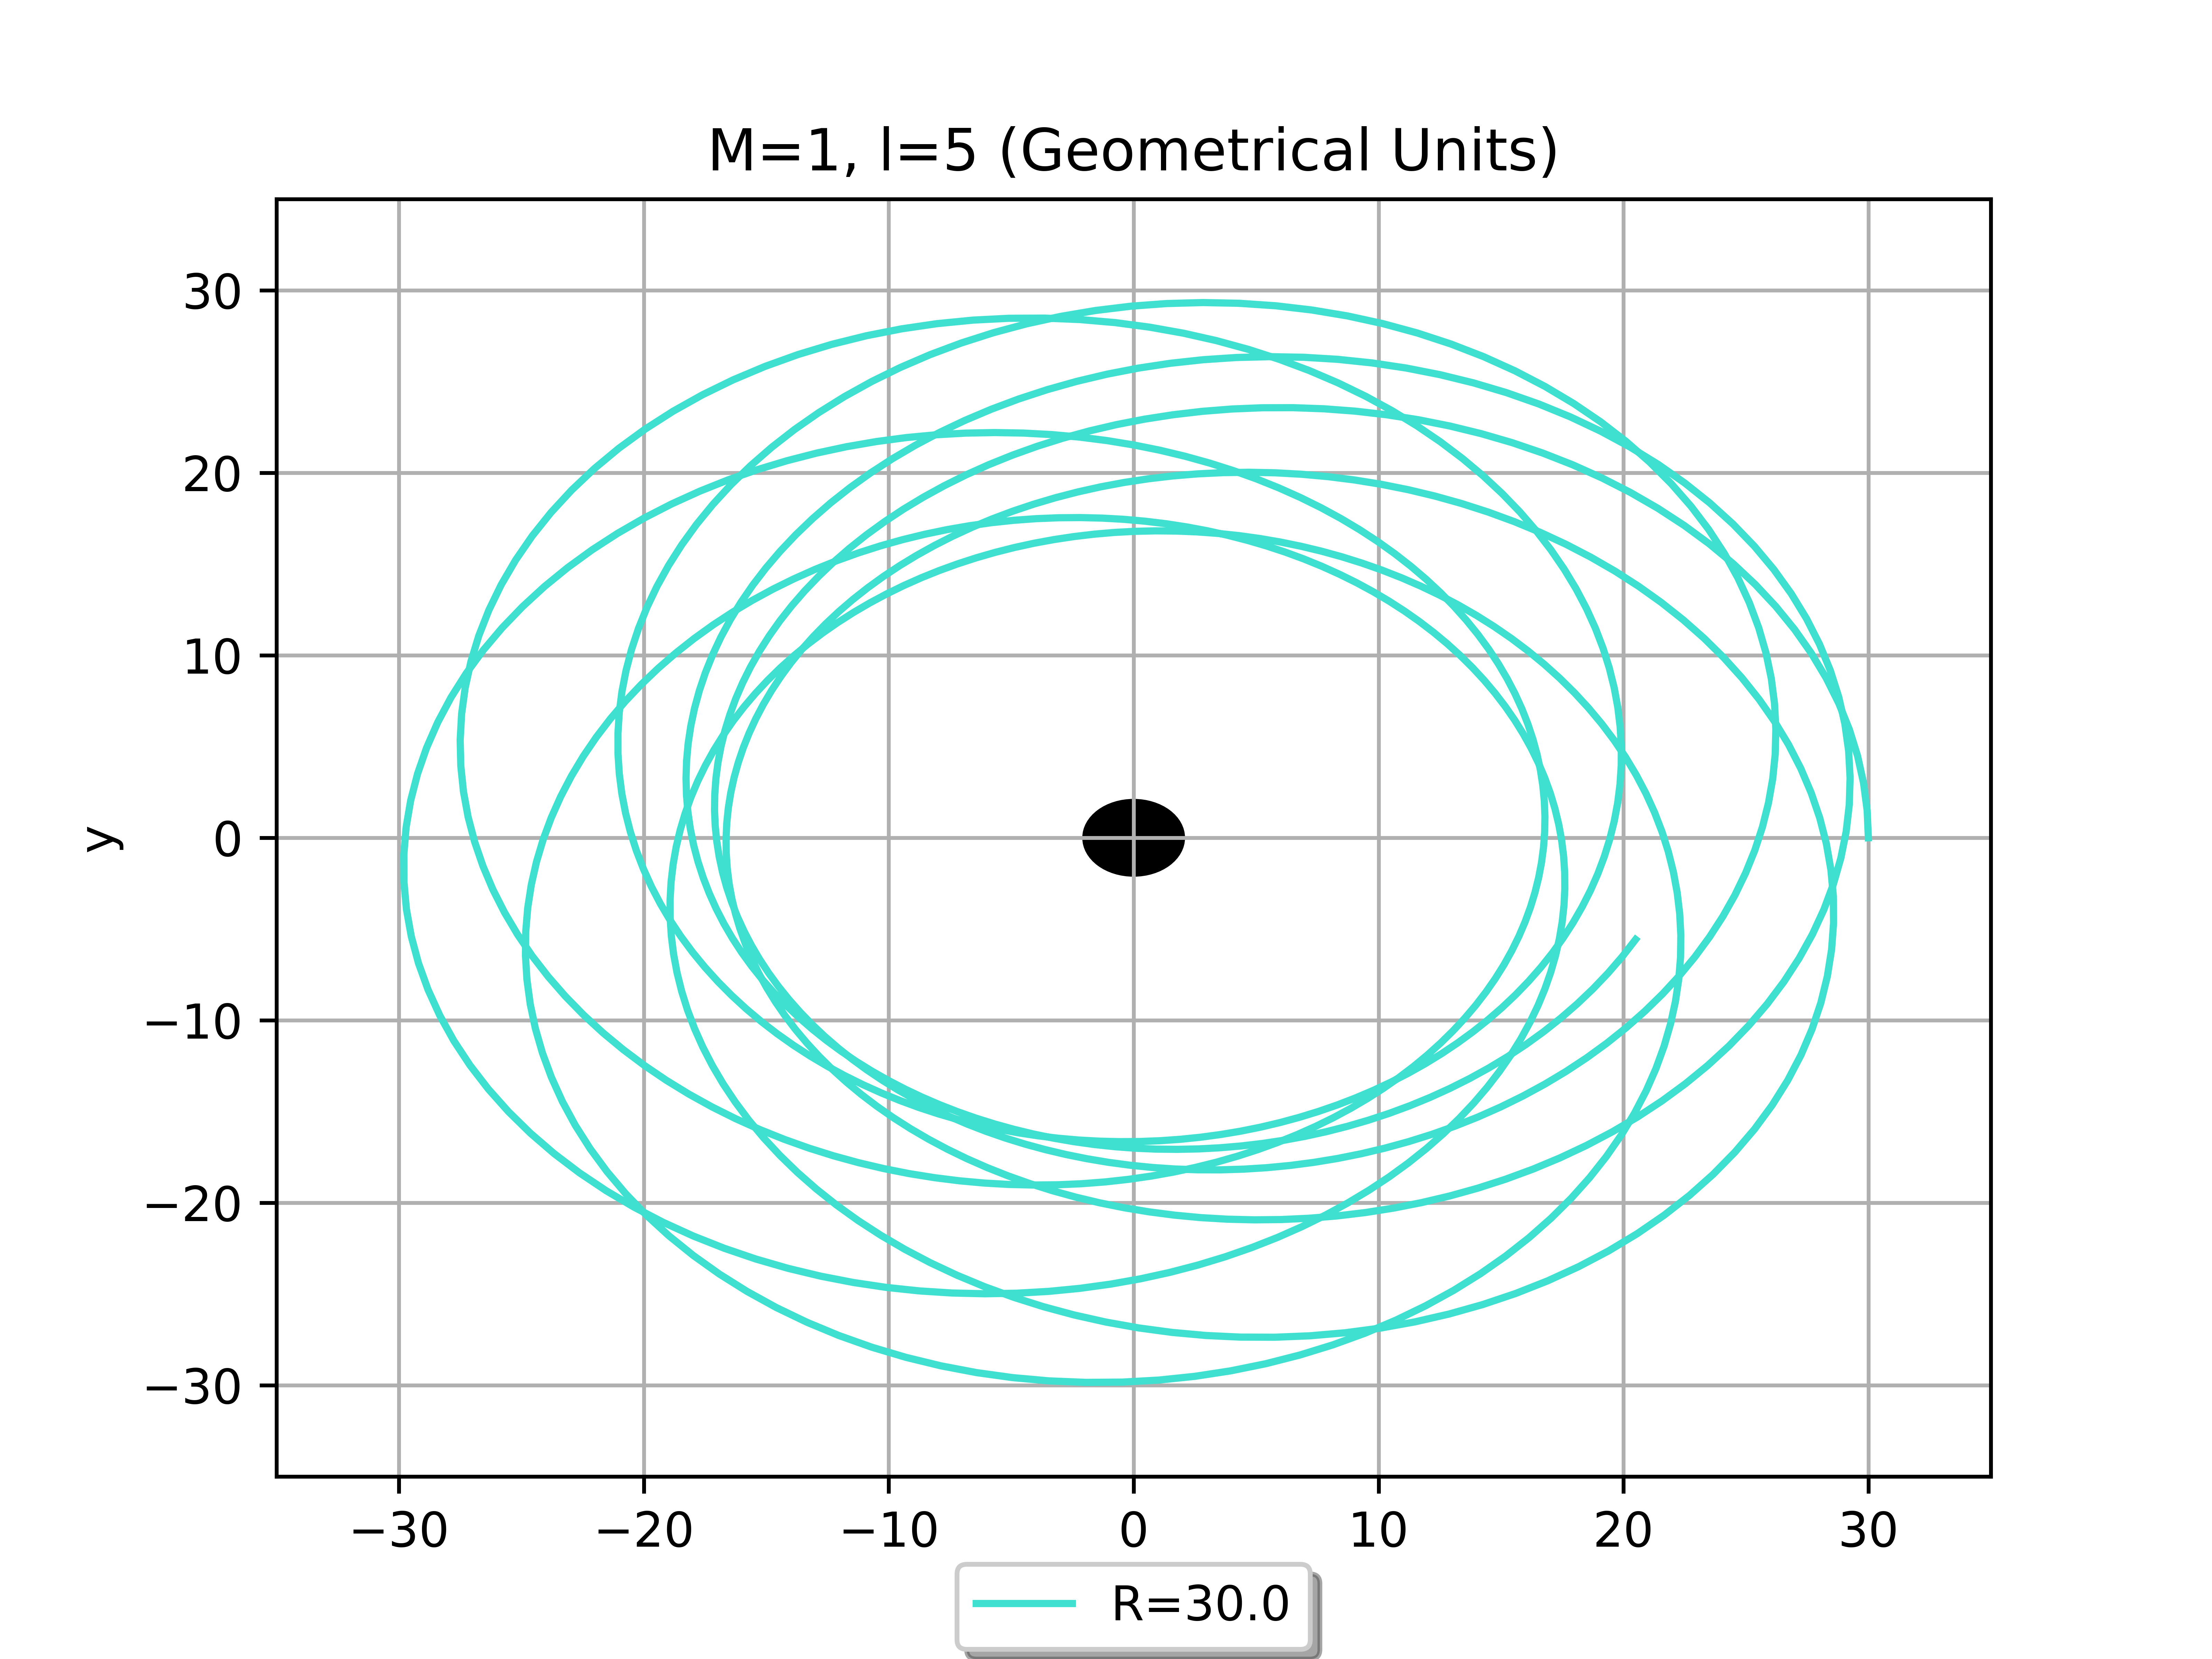
\includegraphics[width=0.9\linewidth, height=6cm]{OrbitS_R=30.png}
\caption{Orbita con condiciones iniciales x=30 e y=0, fuente: elaboración propia.}
\label{fig:ISCO_S2}
\end{subfigure}
\caption{Orbitas en la métrica de Schwarzschild.}
\label{fig:ISCO_S}
\end{figure}

Podemos observar en (Fig: \ref{fig:ISCO_S1}) que usando métrica de Schwarzschild solo las orbitas con radios $R_{+}$ y $R_{-}$ siguen orbitas circulares estables, vemos que si empiezan en un radio intermedio, estos salen despedidos hacia el infinito, si empiezan en un radio inferior a $R_{-}$ estos caen hacia el agujero negro y si empiezan en un radio superior a $R_{+}$, como en (Fig: \ref{fig:ISCO_S2}) estos tendrán una orbita estable pero no circular.

Para la métrica de Kerr tenemos que usar el potencial efectivo (\ref{39}):

\begin{equation}
    \frac{dV}{dr}=\frac{M}{r}+\frac{-(l^{2}-a^{2}(e^{2}-1))}{r^{3}}+\frac{3M(l-ae)^{2}}{r^{4}}=0
\end{equation}

Por lo que nos queda la solución:

\begin{equation}\label{ISCO_Kerr}
    r=\frac{1}{2M}(l^{2}+a^{2}(1-e^{2})+\sqrt{(l^{2}+a^{2}(1-e^{2}))^{2}-12M^{2}(l-ae)^{2}}
\end{equation}

Si volvemos a comprobar ahora volviendo a hacer simulaciones:

\begin{figure}[H]
    \centering
    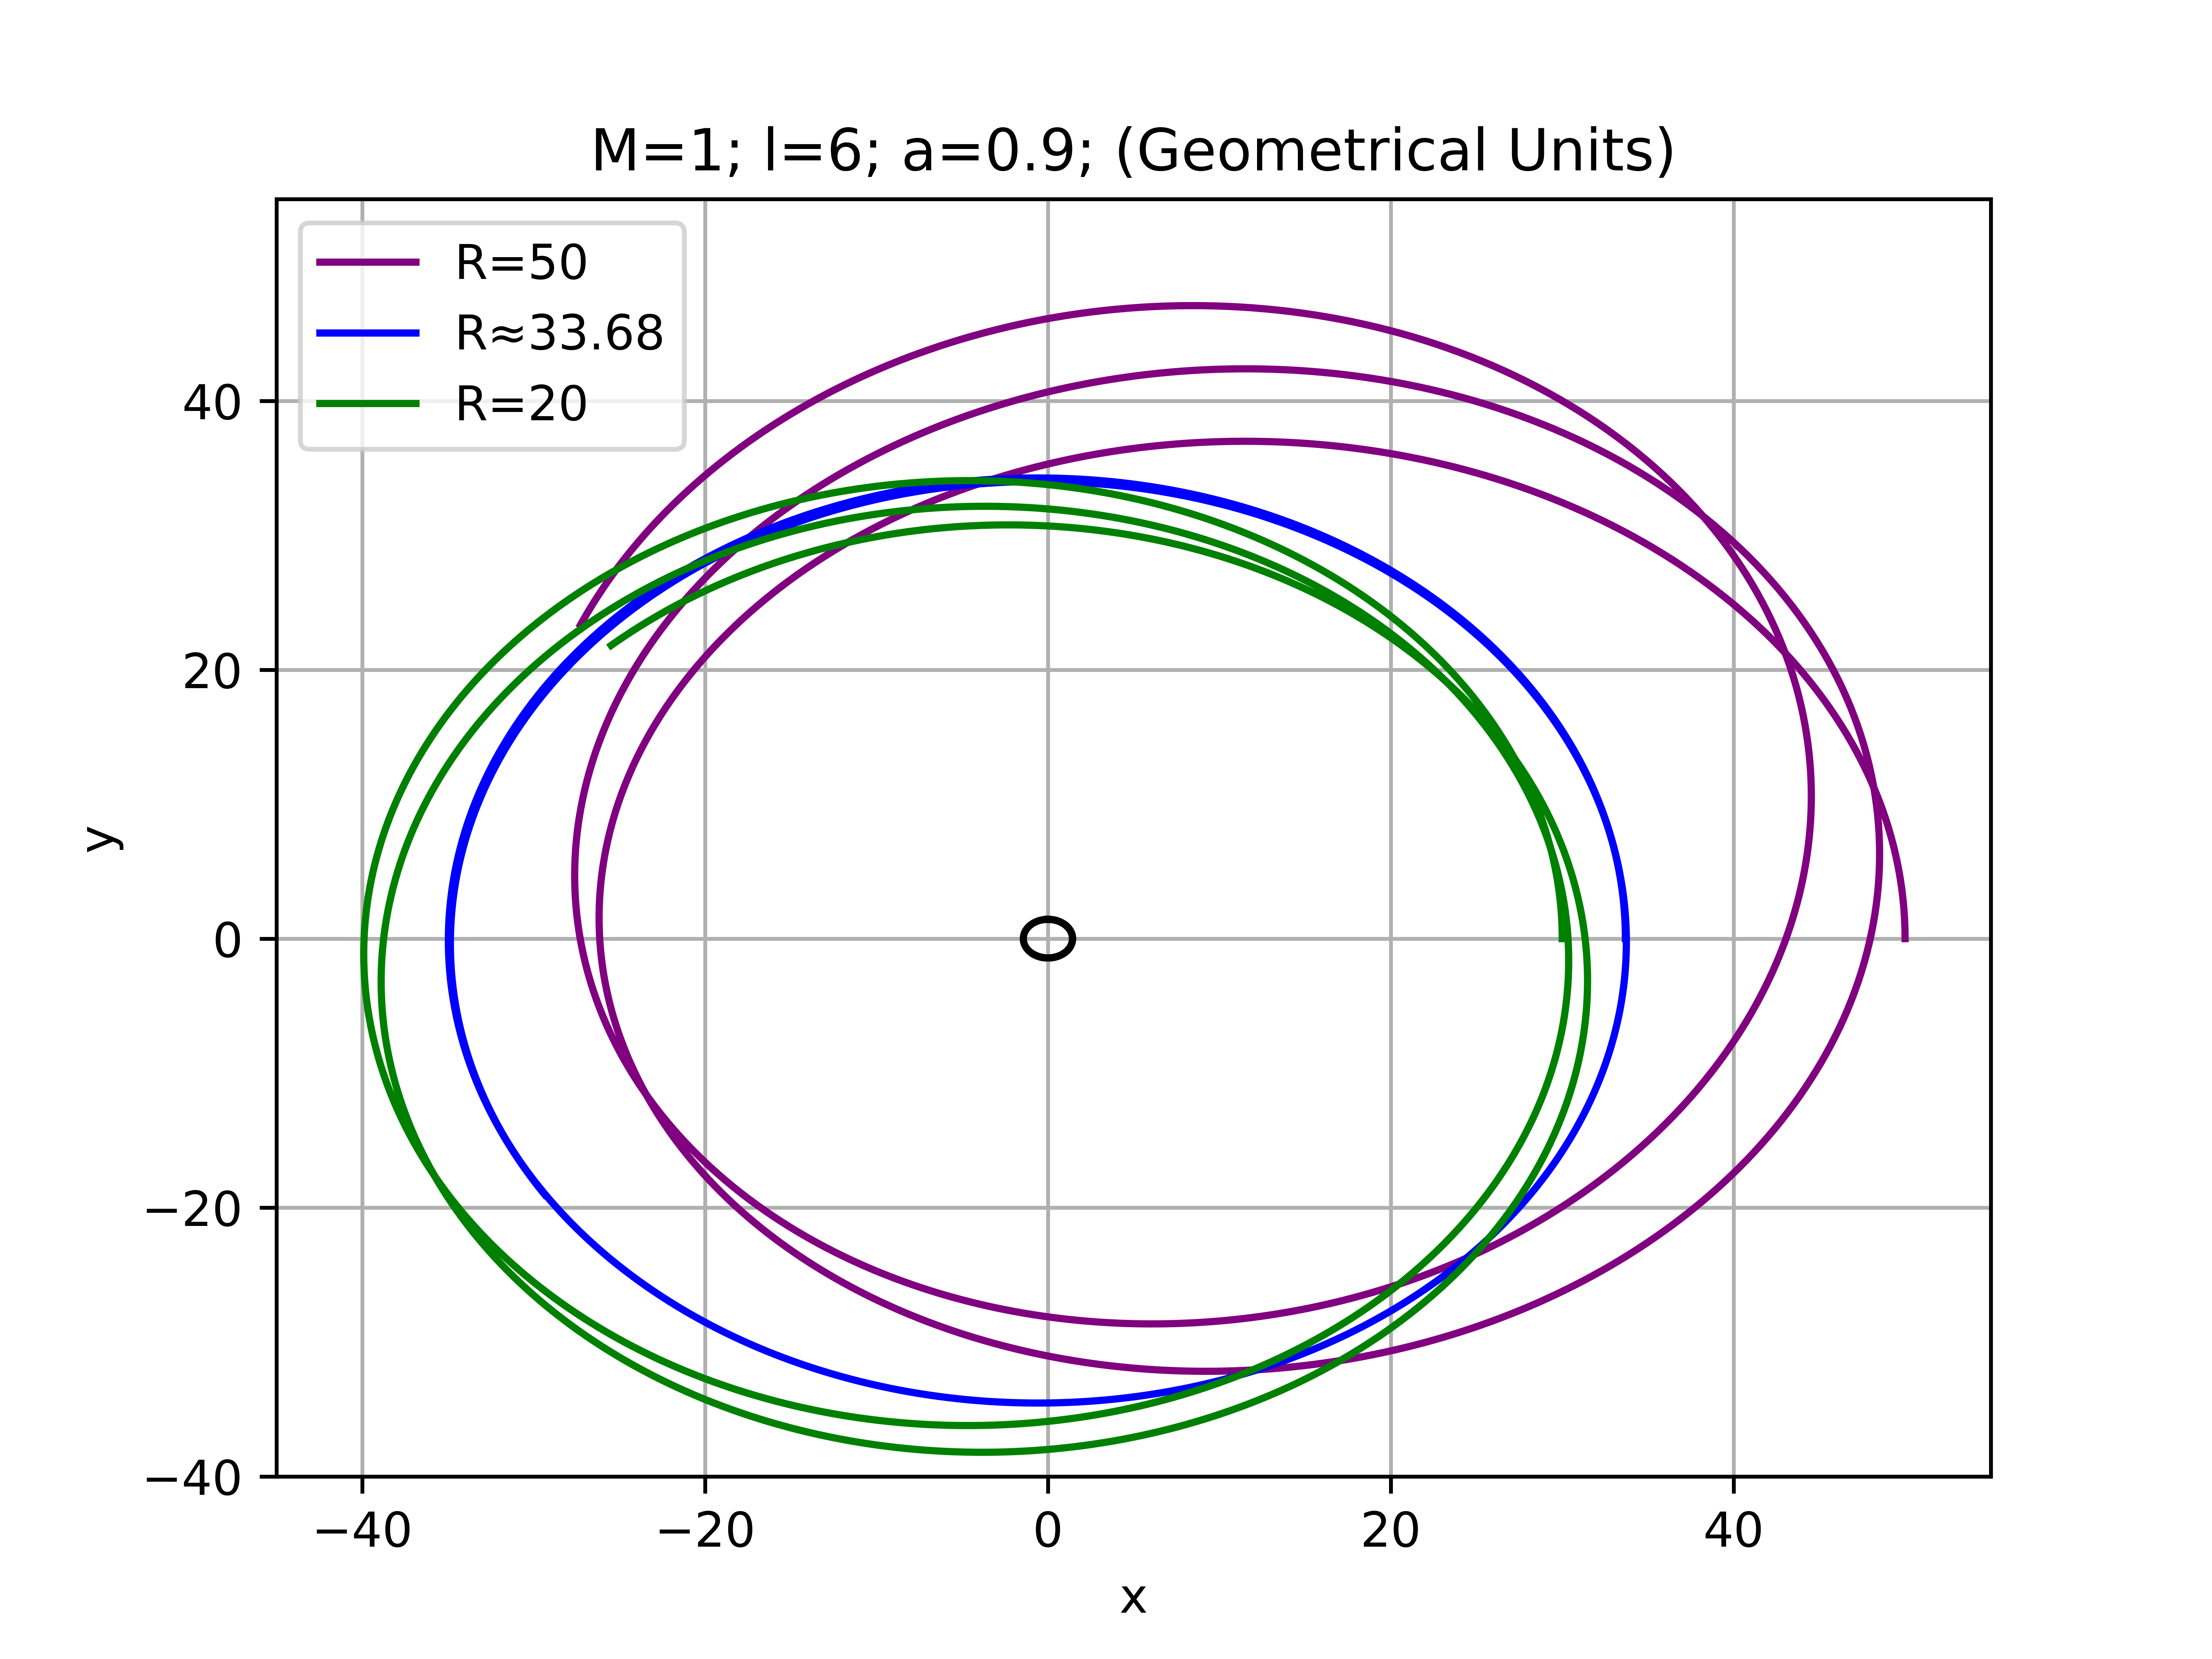
\includegraphics[width=0.7\linewidth]{ISCO_Kerr.png}
    \caption{ISCO comparadas con orbitas inestables en la métrica de Kerr considerando $e=0.999$, fuente: elaboración propia.}
    \label{fig:ISCO_Kerr}
\end{figure}

Se puede observar en (Fig: \ref{fig:ISCO_Kerr}), que en el radio $R\approx33.68$ la orbita es circular estable como se obtendría usando la ecuación (\ref{ISCO_Kerr}), para los radios superiores e inferiores aún sigue una orbita aparentemente estable pero no circulares.

\subsection{Ergosfera}
La región entre $r_{+}$ y $s_{+}$ se denomina ergosfera, en esta zona los observadores no pueden permanecer estáticos: sus sistemas de referencia son irremisiblemente arrastrados por la rotación del espacio-tiempo. Sin embargo, esta zona es intermedia entre el exterior y el horizonte de sucesos, por lo que los observadores pueden permanecer o salir de esta zona, sin caer necesariamente hacia la singularidad.\cite{jeffersonagujeros}

En la ergosfera también podemos encontrar un efecto de la curvatura llamado arrastre de sistemas inerciales("frame dragging", en ingles), tiene que ver con el arrastre rotatorio que sufren los sistemas que se aproximan al agujero negro de Kerr, incluso si tienen momento angular nulo. Este efecto no existe en Schwarzschild ya que, se debe al termino $g_{t\phi}$.\cite{jeffersonagujeros}

El efecto de "frame-dragging" nos sugiere que, a partir de cierto punto, la fuerza de arrastre sera tal que no habrá ningún sistema capaz de mantenerse estático respecto a un observador lejano y se vera obligado a acompañar al agujero negro en su giro. Esto supone, por supuesto, que en ese punto se encuentra la superficie de límite estacionario.\cite{jeffersonagujeros}

\subsubsection{El Proceso de Penrose}
Roger Penrose se dio cuenta de que se podía extraer energía de la ergosfera.

El proceso es de esta manera; una particula con un cuadrimomento $p^{\mu}$ se divide en dos particulas $p^{\mu}=p^{\mu}_{A}+=p^{\mu}_{B}$, $E=E_{A}+E_{B}$ de tal forma que una de esas partículas tiene una energía negativa $p^{\mu}_{A} < 0$ y el otro escapa hacia el infinito, el primero es tragado por el agujero negro (cruza el horizonte de eventos) mientras que el segundo lleva mas energía que la partícula original $p^{\mu}_{B} > p^{\mu}$. Por lo que parte de la energía del agujero negro ha sido extraída.\cite{penrose1971extraction}

\begin{figure}[H]
    \centering
    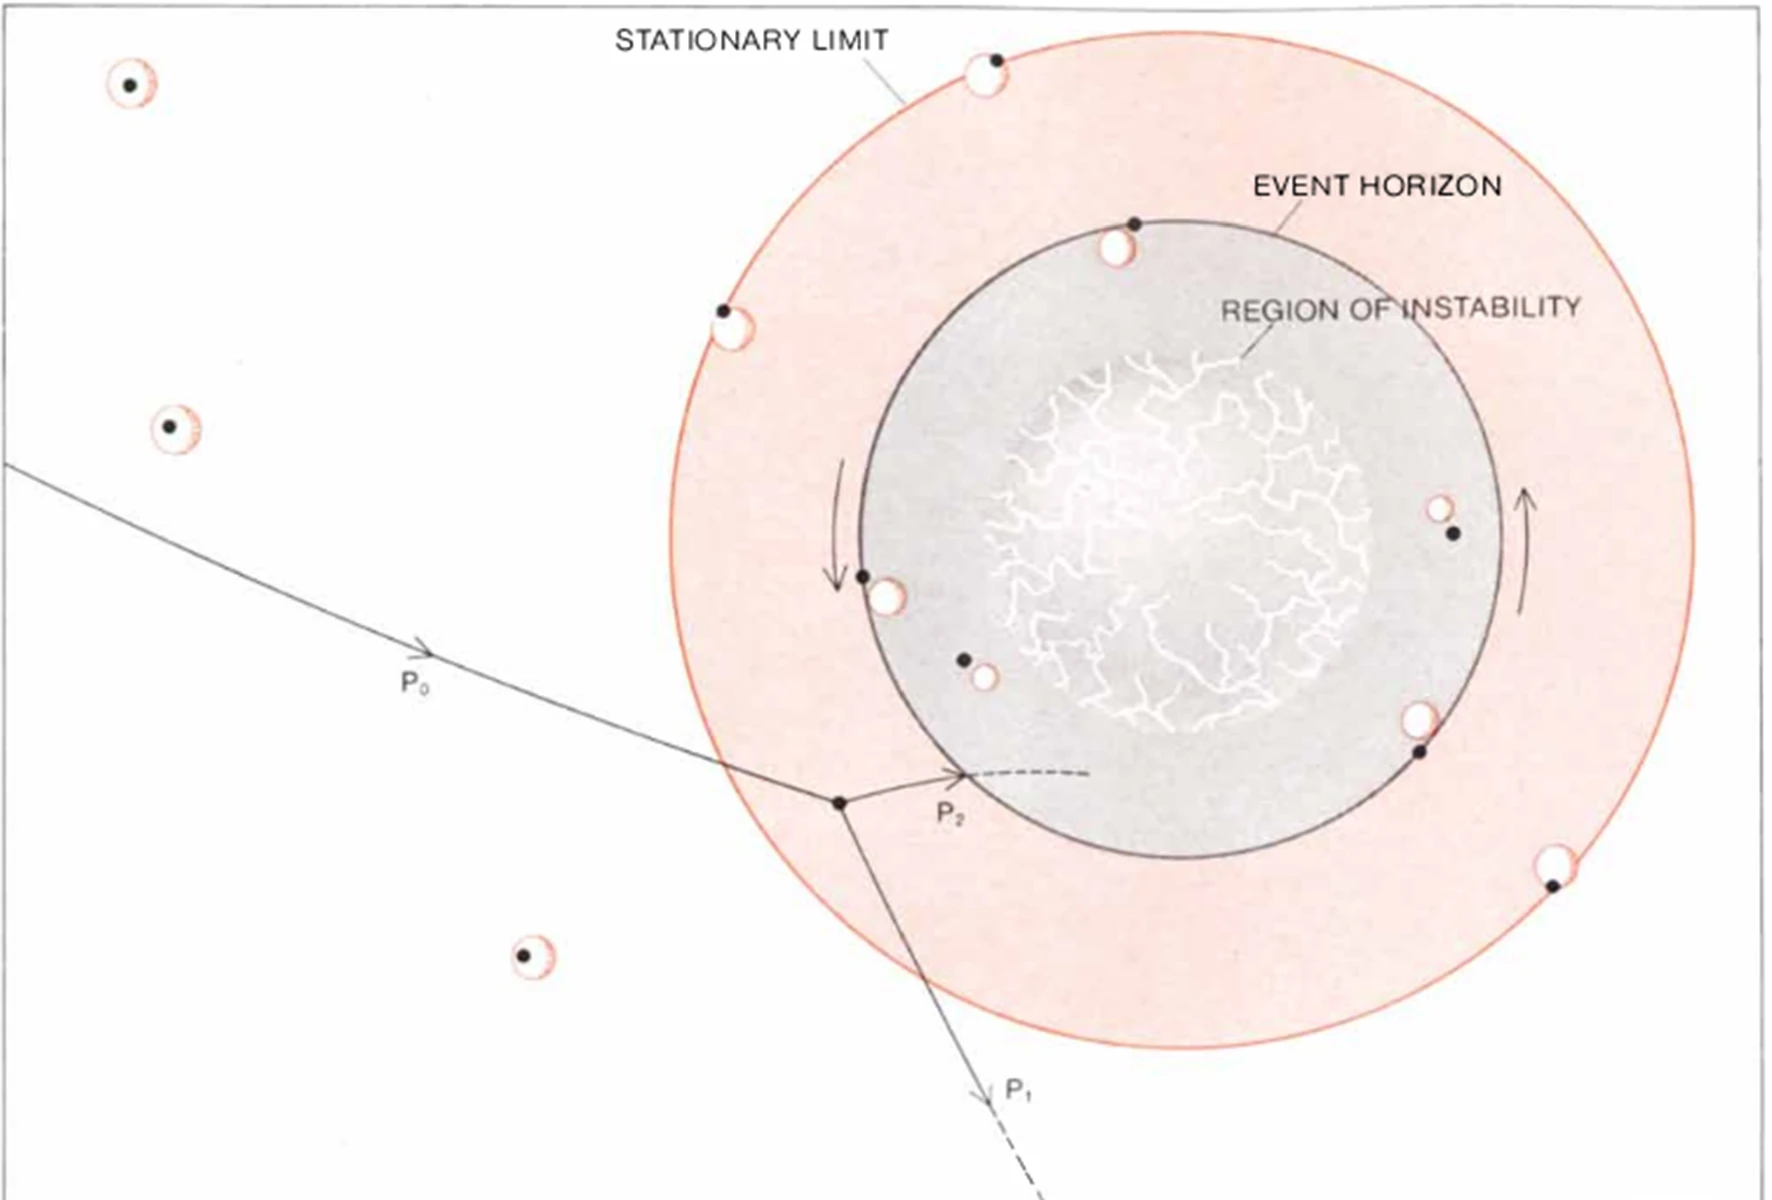
\includegraphics[width=0.5\textwidth]{PenroseProcess.png}
    \caption{Proceso de  Penrose, fuente: \cite{almeida2021thermodynamics}.}
    \label{fig:PenroseProcess}
\end{figure}

En (Fig: \ref{fig:PenroseProcess}) la partícula entra en la ergosfera y se divide en las partículas 1 y 2, la partícula 2 cae en el agujero negro mientras que la partícula 1 sale de la ergosfera con mas energía que la partícula original.

\subsubsection{Termodinámica de los Agujeros Negros}
En astrofísica el teorema de "no-cabello" formula: 'En teoría gravitacional estándar, la geometría exterior del agujero negro mas general está dada por la solución de Kerr-Newman con M, Q y J como únicos parámetros'.\cite{garcia2007termodinamica}
Toda información adicional de la materia que lo formó al agujero cae en él, desaparece tras el horizonte de eventos y es por tanto permanentemente inaccesible a observadores externos, de hecho si hubieran dos agujeros negros, uno de materia y otro de antimateria, serían completamente indistinguibles.\cite{garcia2007termodinamica}

Si calculamos el área de un agujero negro de Kerr obtendríamos:\cite{teukolsky2015kerr}

\begin{equation}\label{AreaKerr}
    A=8\pi Mr_{+}
\end{equation}

Donde $r_{+}=M+\sqrt{M^{2}-a^{2}cos^{2}\theta}$, reemplazando a por $J=aM$ y diferenciando, obtenemos:\cite{teukolsky2015kerr}

\begin{equation}\label{23}
    \delta M=\frac{1}{8\pi}\kappa \delta A+ \Omega \delta J
\end{equation}

donde,

\begin{align}
    \kappa=\frac{r_{+}-M}{2A}&&\Omega=\frac{a}{2Mr_{+}}
\end{align}

Aquí $\Omega$ es la velocidad angular del horizonte y $\kappa$ es la superficie gravitatoria, relacionado con la aceleración de la partícula que gira con el agujero negro en el horizonte.\cite{teukolsky2015kerr}

Si observamos la ecuación (\ref{23}) podemos notar que es muy similar al primer principio de la termodinámica donde si A es proporcional a la entropía entonces $\kappa$ es proporcional a la temperatura.\cite{teukolsky2015kerr}

En el tratamiento clásico, las leyes mecánicas de los agujeros negros se consideraban analogías con las leyes reales de la termodinámica. Dado que se suponía que los agujeros negros no podían radiar ya que se les consideraba a temperatura cero, esto significaba que $\kappa$ no podía ser su temperatura real. Todo esto cambia cuando Hawkings descubre que cuando consideramos efectos cuánticos, un agujero negro puede radiar y esa radiación era térmica y con una temperatura:\cite{teukolsky2015kerr}

\begin{equation}
    T=\frac{\hbar\kappa}{2\pi}
\end{equation}

Esta ecuación es muy importante ya que es la primera que usa tanto la física cuántica como la relatividad general y nos puede dar una pista para unificar las dos teorías.

\section{Agujeros negros astrofísicos}

Hasta ahora hemos estado estudiando los agujeros negros que son consecuencia de las ecuaciones de campo de Einstein y de la relatvidad general, podríamos pensar incluso que son una consecuencia teórica sin ningún tipo de evidencia real, pero los agujeros negros son un objeto astrofísico real que causa efectos evidentes en su entorno y que nosotros podemos estudiar.

\subsection{Evidencias observacionales}
Los agujeros negros al no ser emisores de luz, no podemos observarlos en si mismos, pero hay varios métodos para detectarlos. Unos se denominan directos, en los que  y otros indirectos, ya que el observador no se preocupa del agujero negro en si, si no en sus efectos.\cite{muller2007experimental}El principal problema para detectarlos es diferenciarlos de otros objetos supermasivos que puedan provocar unos efectos gravitatorios parecidos, la diferencia es que son los agujeros negros los que llegan a cotas tan altas de masa.

\subsubsection{Método cinético}
Una manera de detectarlos indirectamente es el método cinética, la idea es sencilla debido al movimiento de los objetos que sienten un potencial gravitacional muy fuerte debido al agujero negro podemos obtener sus propiedades, como su masa o su espín.\cite{muller2007experimental}

En la practica se utiliza cualquier objeto luminoso como estrellas que puedan ser visibles desde la Tierra del que podamos obtener su trayectoria, normalmente siguiendo una orbita kepleriana. El primer agujero negro fue detectado en 1971, en el que Tom Bolton estudiando el sistema binario Cygnus X-1 formado por una estrella gigante y un objeto compacto, midiendo la velocidad de la estrella gigante O–star HDE 226868 determinó la masa de la compañera siguiendo el método cinético, descartando otras posibilidades como una enana blanca o una estrella de neutrones.\cite{muller2007experimental}

\begin{figure}[H]
    \centering
    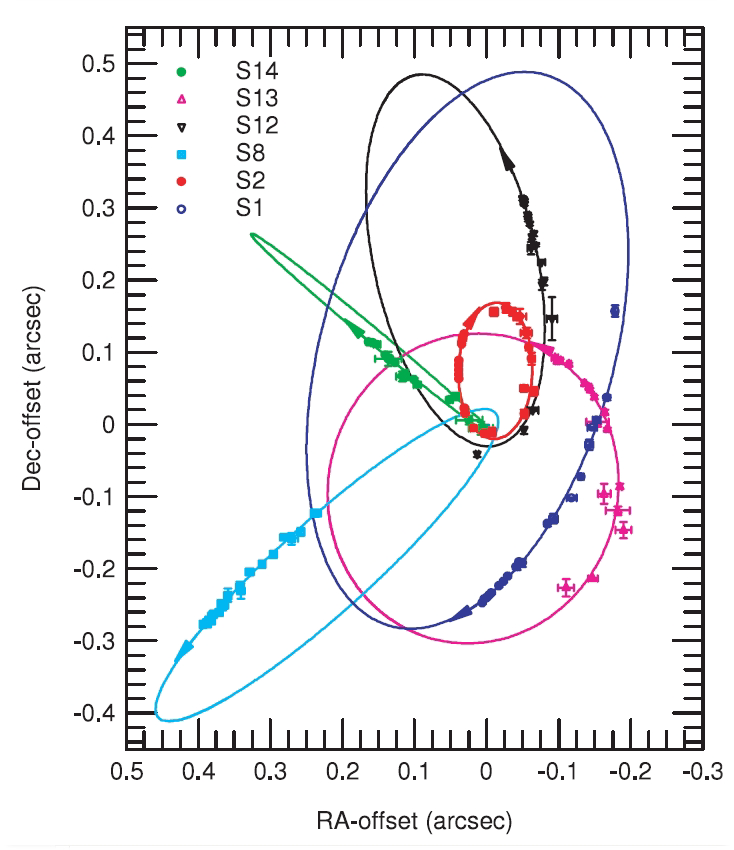
\includegraphics[width=0.5\textwidth]{SixStarsOrbits_Genzel.png}
    \caption{Trayectoria de seis objetos luminosos orbitando el agujero negro Sgr A*, fuente: \cite{genzel2005sinfoni}.}
    \label{fig:SixStarsOrbits_Genzel}
\end{figure}

Uno de los grandes trabajos aplicando este método cinético fue el descubrimiento del agujero negro Sagitario A* en donde, como se puede ver en (Fig: \ref{fig:SixStarsOrbits_Genzel}), siguiendo la trayectoria de seis estrellas diferentes que lo orbitaban, pudieron determinar sus características.\cite{muller2007experimental}

\subsubsection{Métodos espectro-relativistas}
Este método trata de observar los efectos relativistas de las lineas espectrales cuyo emisor se encuentre lo suficientemente cerca del agujero negro.\cite{muller2007experimental}

Los efectos que se observarían en las lineas espectrales son varios, para empezar se produciría el efecto Doppler; en la parte del disco del agujero negro que decelera se detectaría un corrimiento al rojo y un corrimiento al azul en la parte en la que acelera hacia el observador.\cite{muller2007experimental}

Además debido a la gran inclinación hay un efecto radiante debido a la relatividad especial.\cite{muller2007experimental}

En tercer lugar, el agujero negro captura fotones lineales debido a la fuerte curvatura espacio-temporal, las lineas espectrales sufren un corrimiento al rojo.\cite{muller2007experimental}

\begin{figure}[H]
    \centering
    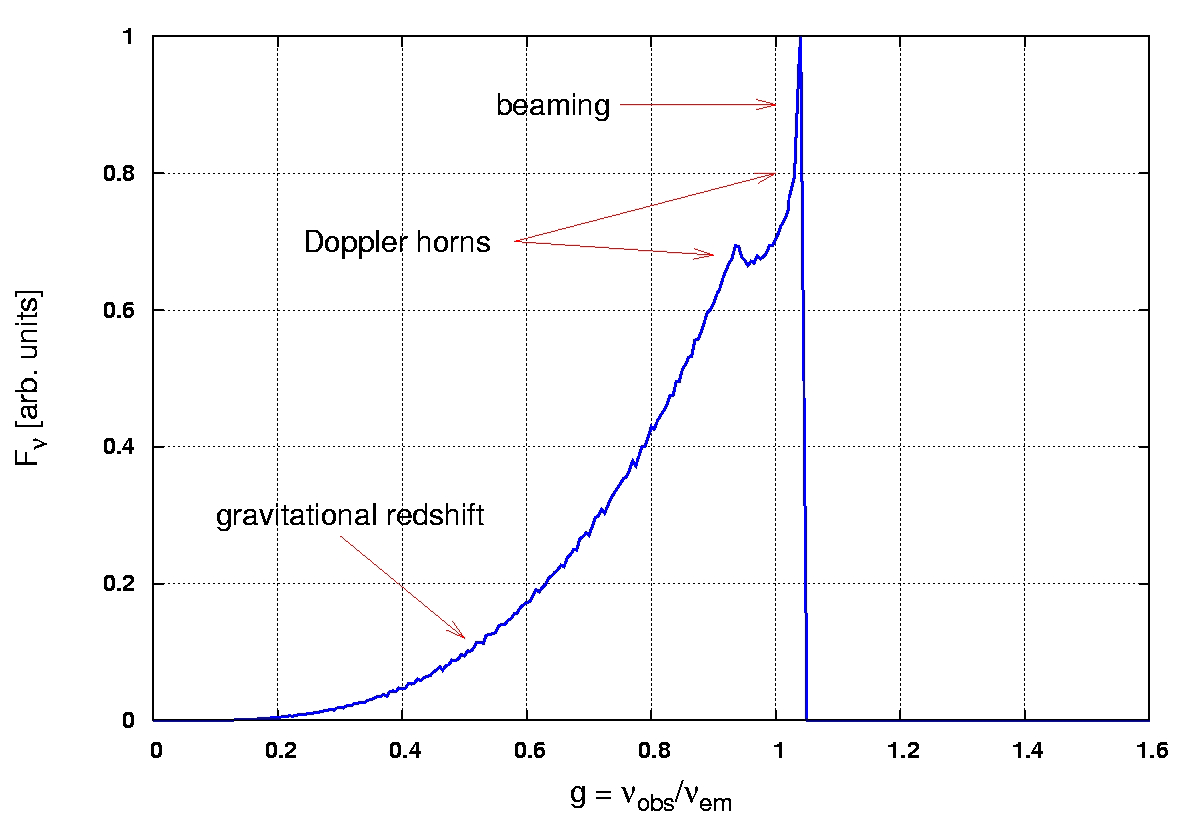
\includegraphics[width=0.6\linewidth]{spectral-relativist_effect.png}
    \caption{Prototipo de línea espectral relativista sometido a los tres efectos antes mencionados, fuente: \cite{muller2007experimental}.}
    \label{fig:spectral-relativist_effect}
\end{figure}

Un ejemplo de este método es la figura (Fig: \ref{fig:spectral-relativist_effect}).

\subsubsection{Método de acreción}
Los agujeros negros supermasivos que se encuentran en el centro de la galaxia se denominan AGN(Nucleo Activo de la Galaxia), estos se encuentran rodeados de mucha materia a su alrededor que está cayendo hacia ellos y es acelerada por el agujero negro, por eso es interesante desarrollar un método nuevo relacionado con esto, el método de acreción, que consiste en estudiar los efectos luminosos causados por la materia que ha sido acelerada por el agujero.\cite{muller2007experimental}

Esta materia fluye por la inestabilidad hacia el centro del AGN, de esta manera se forma un flujo de acreción plano llamado disco de acreción estándar. En las proximidades del agujero negro supermasivo surgen efectos magnéticos que impulsan fuertes salidas, los jets. La parte teórica que estudia los jets en los agujeros negros supermasivos se denomina GRMHD (general relativistic magnetohydrodynamics).\cite{muller2007experimental}

Se puede utilizar la relación de Eddington que relaciona la luminosidad a la tasa de acreción y a la masa del agujero negro, los métodos de acreción son de particular interés para tasas de acreción altas.\cite{muller2007experimental}

\subsubsection{Método eruptivo}
El método eruptico está asociado a la emisión de alta energía. Estos fenómenos son comunes en la astronomía y la complejidad es escoger cuales de estos están asociados a un agujero negro.\cite{muller2007experimental} 

Los que mas pueden estar relacionados son los llamados grandes emisores de rayos gamma (GRB, Gamma–ray bursts); estos son eventos breves en los que se inunda completamente el cielo casi oscuro con su radiación de rayos gamma. De hecho, son las explosiones electromagnéticas más concentradas y brillantes del Universo.\cite{meszaros2006gamma} Los astrofísicos están convencidos de que en cada GRB se forma un agujero negro de masa estelar e impulsa chorros ultrarelativistas\cite{muller2007experimental} 

El evento de disrupción de marea es también un método eruptivo, este consiste en una estrella se acerca demasiado a un agujero negro, la estrella al principio es deformada por las fuerzas de marea del agujero negro, las cuales superan la propia gravedad de la estrella, llega un punto en el que la estrella es desintegrada por le agujero negro, sus restos se quedan esparcidos cerca del agujero negro y pueden ser acelerados en parte.\cite{muller2007experimental}

\begin{figure}[H]
    \centering
    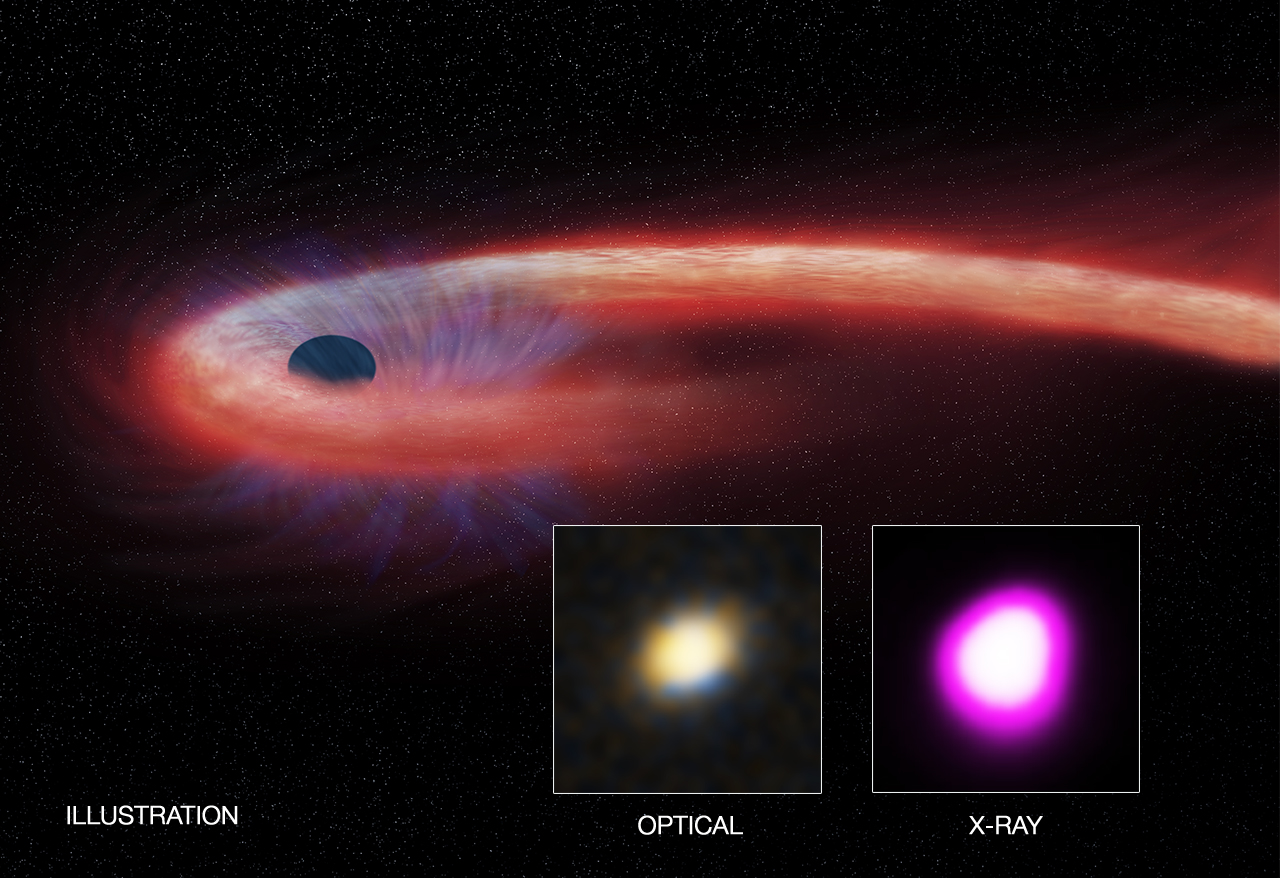
\includegraphics{Tidal disruption events NASA.jpg}
    \caption{Representación artística de una disrupción de marea, fuente: \href{https://www.nasa.gov/mission_pages/chandra/multimedia/artists-illustration-of-tidal-disruption-event.html}{NASA}.}
    \label{fig:Tidal disruption events NASA}
\end{figure}

Una ilustración artística (Fig: \ref{fig:Tidal disruption events NASA}) muestra como una estrella está siendo absorbida por un agujero negro.

\subsubsection{Método de las aberraciones}
Este efecto está asociado al hecho de que los agujeros negros causan fuertes efectos de lente gravitacional. Esto significa que la apariencia visual de un objeto cercano a un agujero negro está en general distorsionado.\cite{muller2007experimental}

Gracias a las ecuaciones de las geodésicas nulas se pueden obtener los caminos que va a seguir los fotones debido a la métrica y se pueden simular las imágenes que se deberían encontrar en las observaciones, con estas observaciones podríamos estimar las características del agujero negro.Sin embargo, la resolución de los telescopios no son suficientes para detectar estas distorsiones, aunque algunas ya son posibles de detectar.\cite{muller2007experimental} 

\begin{figure}[H]
\begin{subfigure}{0.5\textwidth}
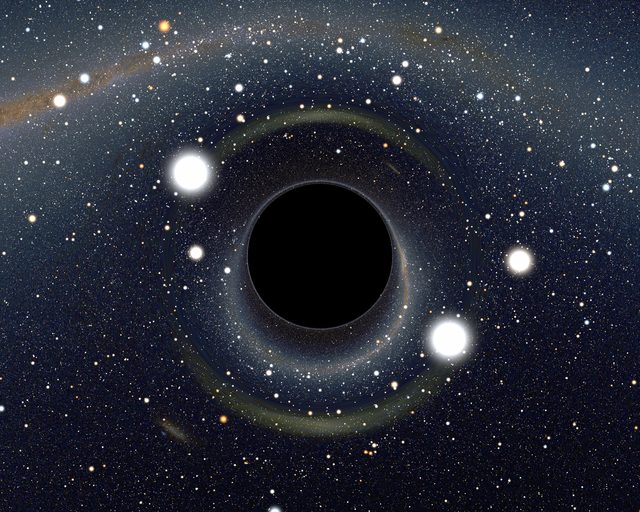
\includegraphics[width=0.9\linewidth, height=6cm]{dobleEstrella_Alain.png} 
\caption{Imagen simulada en la que una misma estrella aparece como dos estrellas, a la misma distancia pero en posiciones opuestas respecto al agujero negro, fuente: \cite{riazuelo2019seeing}.}
\label{fig:dobleEstrella_Alain}
\end{subfigure}\hspace{1cm}
\begin{subfigure}{0.5\textwidth}
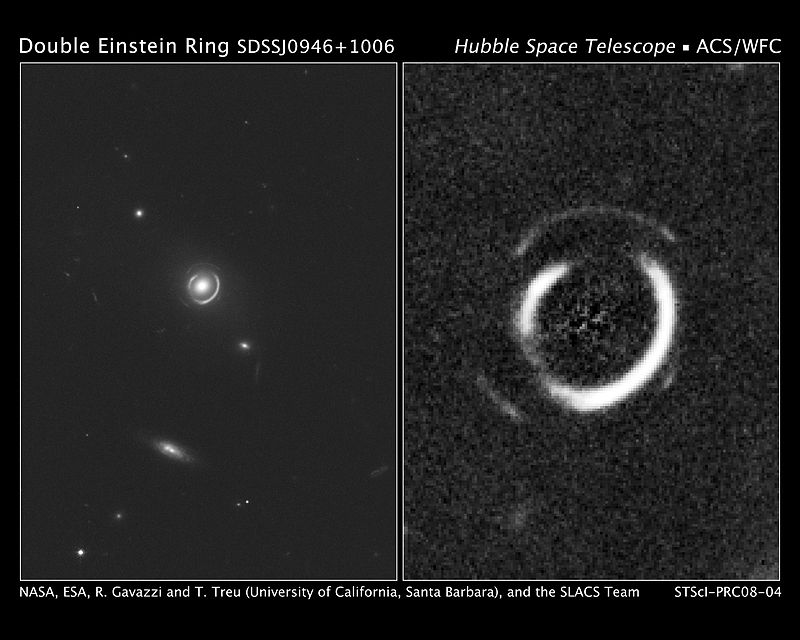
\includegraphics[width=0.9\linewidth, height=6cm]{DoubleEinsteinRing.jpg}
\caption{Anillo de Einstein doble, en este caso producido por una galaxia, detectado por el Hubble Space Telescope.}
\label{fig:DoubleEinsteinRing}
\end{subfigure}

\caption{Efectos Ópticos debido a la métrica.}
\label{fig:image2}
\end{figure}
Algunos de estos efectos ópticos son desdoblamientos de objetos como en (Fig: \ref{fig:dobleEstrella_Alain}) o los anillos de Einstein como en (Fig: \ref{fig:DoubleEinsteinRing}), en los que bajo la circunstancia especial de que la lente gravitacional, la fuente y el observador estén alineados.  
\subsubsection{Método temporal}
Los métodos temporales se basan en el hecho de que la gravedad también provoca efectos de dilatación del tiempo. La fuerte gravedad de los agujeros negros es responsable de los efectos de la dilatación significativa del tiempo. Junto con el efecto de corrimiento al rojo gravitacional, un observador externo establece que 'un reloj luminoso' que cae se vuelve rojo y débil cuando se acerca al agujero combinado con una desaceleración del segundero.\cite{muller2007experimental}

Para que este método funcione tiene que ocurrir algún evento que sepamos que es periódico, en la vecindad del agujero negro.\cite{muller2007experimental} 

Un ejemplo de esto es cuando se reportó variabilidades gigantes y rápidas de rayos X para una galaxia Seyfert-1 de línea estrecha. Estas observaciones son consistentes con fuertes efectos relativistas que tienen impacto en la curva de luz de rayos X.\cite{muller2007experimental} 

\subsubsection{Método por onda gravitacional inducida}
La idea es que el efecto de un objeto compacto en un cuerpo central masivo puede ser utilizado para mapear el espacio-tiempo. Sin embargo, este atractivo concepto está plagado de problemas en la astronomía de ondas gravitacionales, dado que esta parte de la física experimental es muy nueva, ya que hasta hace poco no se habían detectado ondas gravitacionales y no se sabía su forma exacta, además que el emisor de esas ondas no tiene que ser un agujero negro.\cite{muller2007experimental}

En 2016 se detecto la primera onda gravitacional gracias al experimento LIGO, en el que se fusionaron dos agujeros negros que formaban un sistema binario, como se puede apreciar en (Fig: \ref{fig:Experimento LIGO.}).\cite{abbott2017observation} 

Esta onda gravitacional fue medida mediante un interferómetro de Michelson gigante, de 4km cada brazo (Fig: \ref{fig:Michelson}). El experimento consiste en que la onda gravitacional cuando llega, esta se propaga ortogonalmente hacia el plano detector y polarizado linealmente en paralelo a las cavidades ópticas de 4 km, las ondas tendrán el efecto de alargar uno de los brazos del interferómetro y alargar al otro durante un medio ciclo de la onda, estos cambios se revierten en el otro medio ciclo. El fotodetector recoge esta diferencia de longitud de las cavidades.\cite{abbott2017observation} 

Para saber si esta onda fue provocada por dos agujeros negros nos podemos fijar en su masa era de $m_{1}=36M_{\odot}$ $m_{2}=29M_{\odot}$,\cite{abbott2017observation} por lo que podemos suponer que eran tan masivos que se trataban de agujeros negros, ya que la masa máxima de una estrella de neutrones sería de $\approx 3M_{\odot}$.\cite{kalogera1996maximum}

\begin{figure}[H]
\begin{subfigure}{0.5\textwidth}
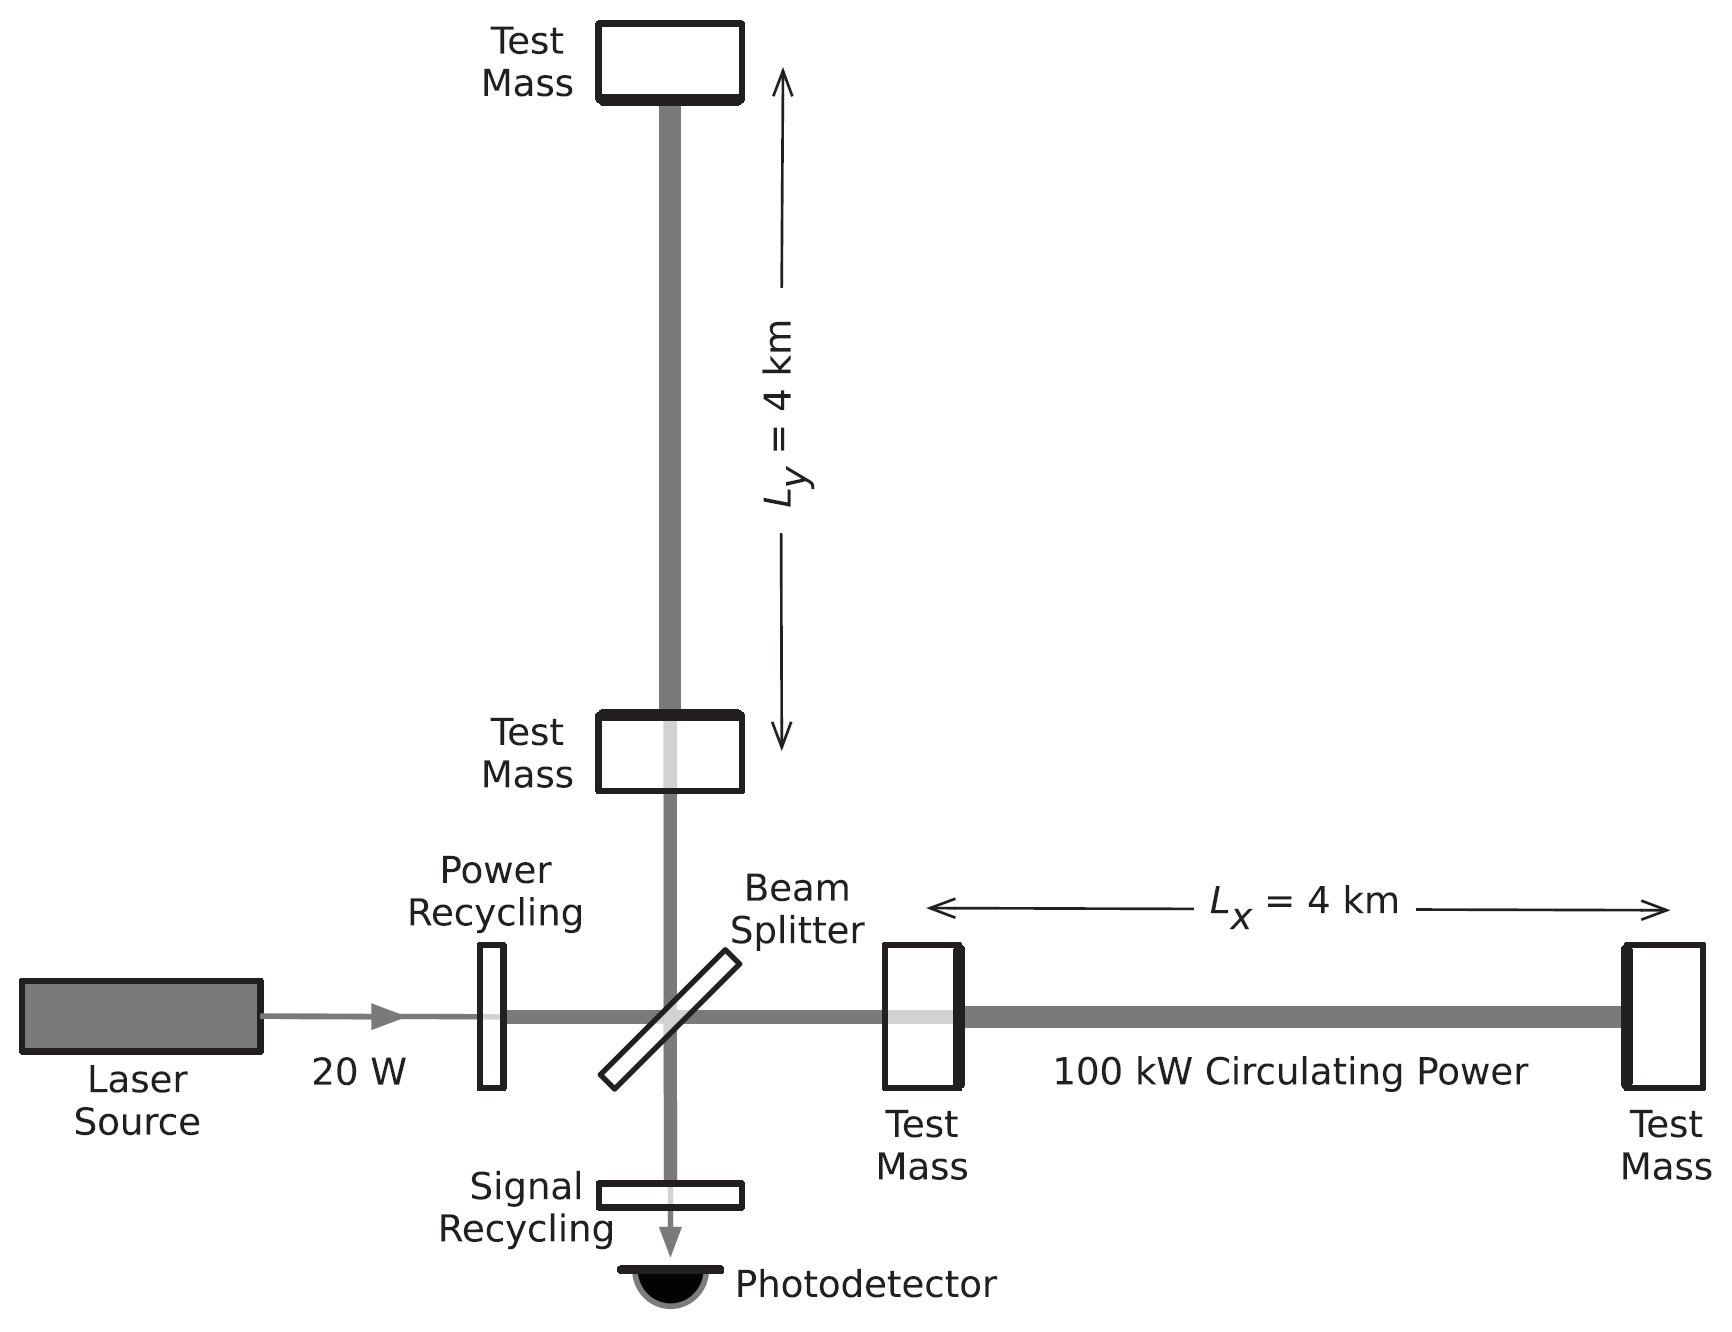
\includegraphics[width=0.9\linewidth, height=6cm]{Michelson_LIGO.png} 
\caption{Interferómetro de Michelson utilizado para detectar la onda gravitacional, fuente: \cite{abbott2017observation}.}
\label{fig:Michelson}
\end{subfigure}\hspace{1cm}
\begin{subfigure}{0.5\textwidth}
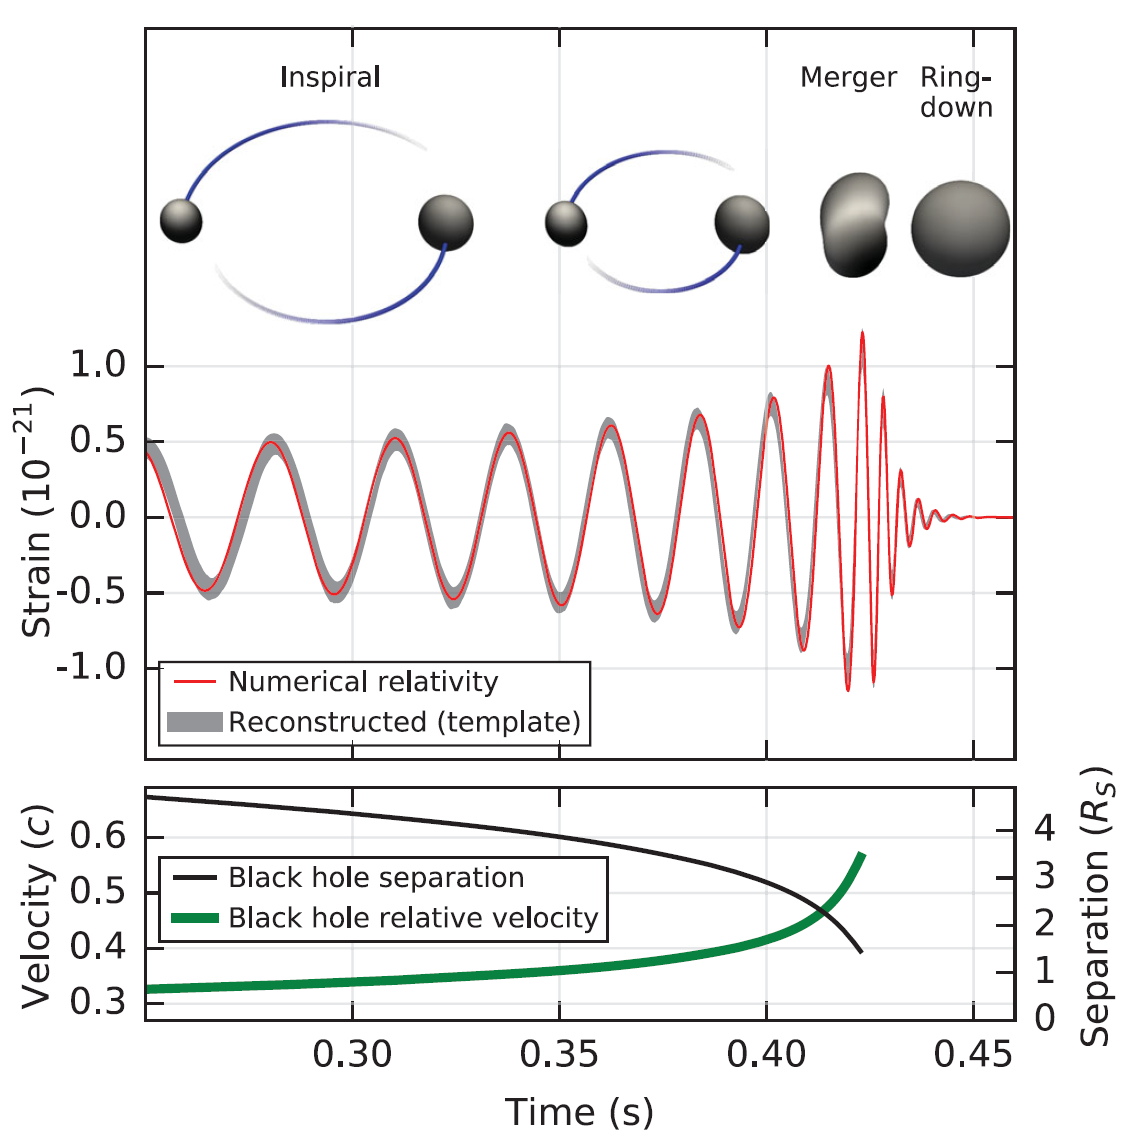
\includegraphics[width=0.9\linewidth, height=6cm]{LIGO.png}
\caption{Estimación del suceso a partir de la onda gravitacional medida, los agujeros negros formaban un sistema doble en el que se iban acercando cada vez mas hasta que se acabaron fusionado, figura obtenida de \cite{abbott2017observation}.}
\label{fig:Experimento LIGO.}
\end{subfigure}
\caption{Experimento LIGO.}
\label{fig:image2}
\end{figure}

\subsubsection{Método del oscurecimiento}
Este método se basa en usar la negritud del agujero negro.\cite{muller2007experimental}

Los agujeros negros no son totalmente esféricos, tienen deformaciones debido al giro que tienen y del ángulo desde el que se les observa. Estas deformaciones se pueden utilizar para determinar las propiedades de los agujeros negros mediante observaciones, estas técnicas aún están por desarrollarse, pero en principio si sabemos la distancia a la que se encuentra el agujero negro y su eje de rotación podríamos saber su espín y su masa.\cite{muller2007experimental}

Una buena analogía sería la imagen de la luna tomando el fondo de rayos X, que emergen alrededor de la mitad negra del disco de la Luna, se puede observar la silueta exacta de la Luna (Fig: \ref{fig:Luna Rosat}).\cite{muller2007experimental}

\begin{figure}[H]
    \centering
    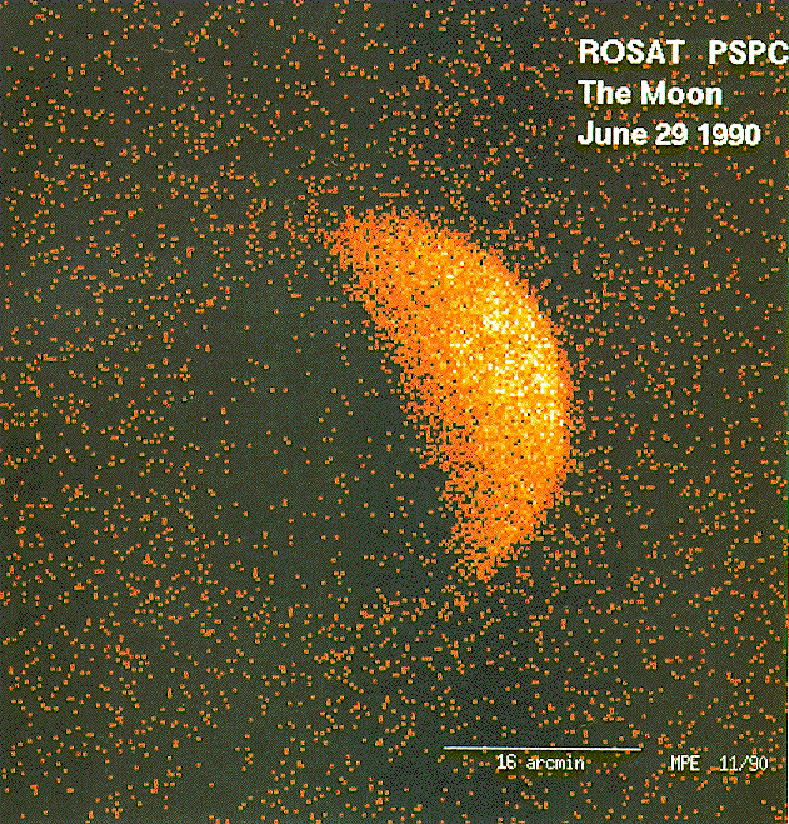
\includegraphics[width=0.5\textwidth]{Luna_ROSAT.png}
    \caption{Silueta de la Luna tomada por ROSAT, fuente: \cite{muller2007experimental}.}
    \label{fig:Luna Rosat}
\end{figure}

Este método de oscurecimiento se utilizó para obtener la "foto" del agujero negro supermasivo M87; (Fig: \ref{fig:M87}).

\subsection{El agujero negro en M87}

\subsubsection{Introducción}
M87 es una galaxia cercana a la nuestra en cuyo centro se encuentra un agujero negro supermasivo M87*, el cual ha cogido especial relevancia en los últimos años ya que ha sido el primer agujero negro "fotografiado", esta fue tomado por la Event Horizon Telescope(EHT).

\subsubsection{Instrumentación y Metodología}
El experimento está formado por una red de telescopios repartidos por toda la tierra, cada uno de estos es un telescopio de interferometría de base muy larga (VLBI) el cual mide directamente la visibilidad, las componentes de Fourier, de la distribución de brillo de radio en el cielo. A medida que la Tierra rota, cada par de telescopios en la red toma muchas muestras de frecuencias espaciales.\cite{event2019firstI}

Para medir las visibilidades interferométricas, Los telescopios, que están ampliamente separados, como se aprecia en (Fig: \ref{fig:EHT}), muestrean simultáneamente y registran coherentemente la campo de radiación de la fuente. Sincronizándose usando el sistema de posicionamiento Global(GPS), logrando la alineación temporal de estas grabaciones en decenas de nanosegundos. Cada estación está equipada con un estándar de frecuencia de máser de hidrógeno.\cite{event2019firstI}

\begin{figure}[H]
    \centering
    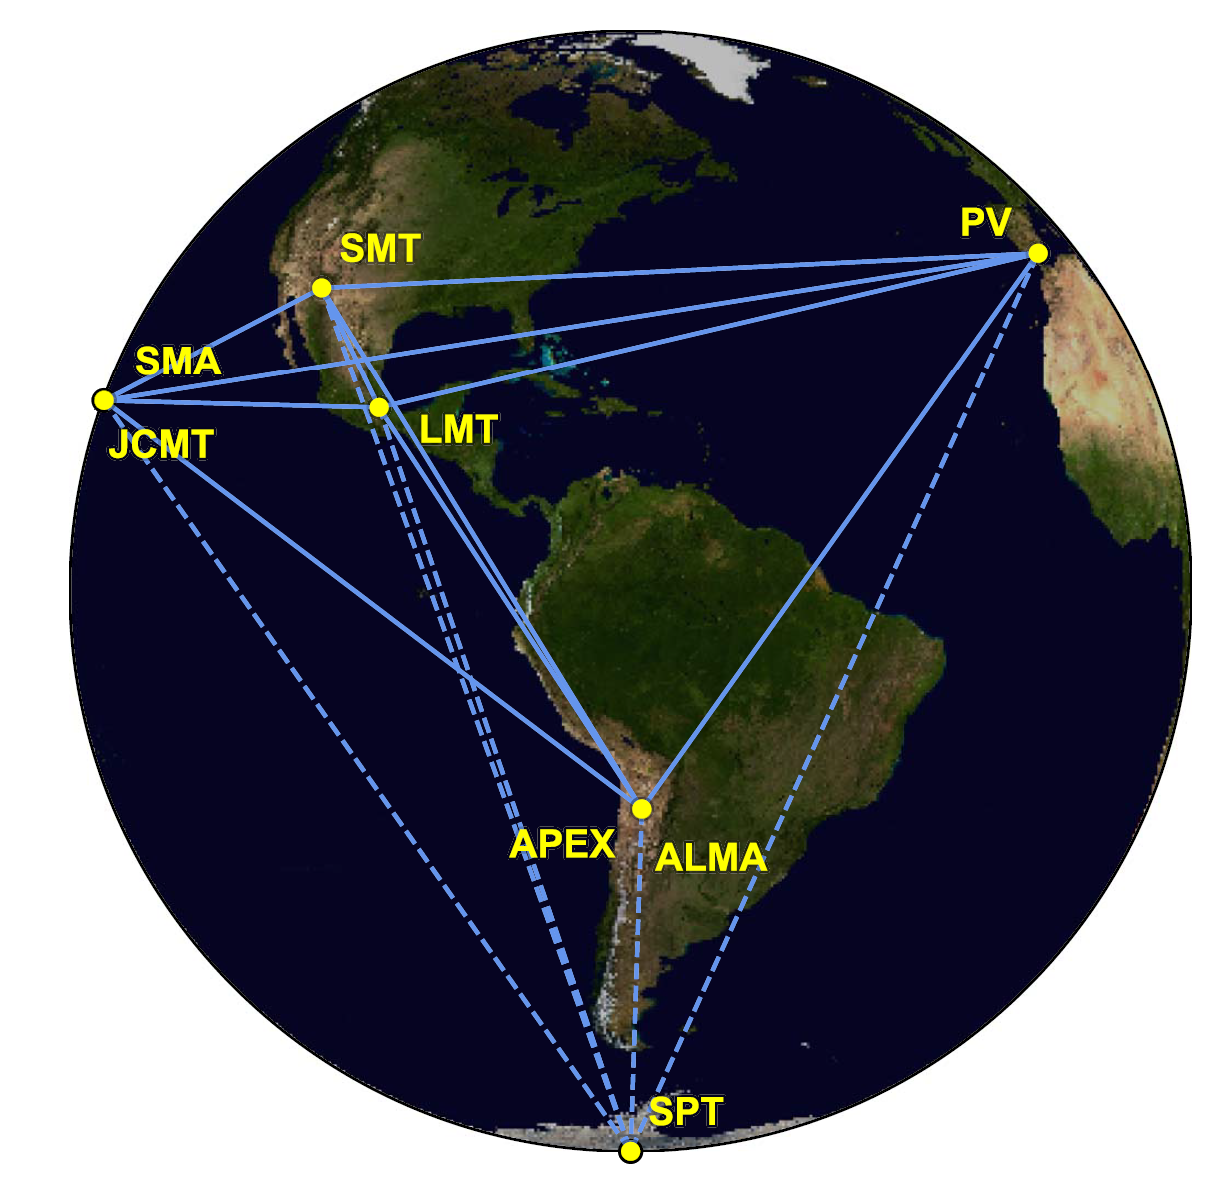
\includegraphics[width=0.5\textwidth]{EHT.png}
    \caption{Ocho estaciones del EHT en seis localizaciones geográficas distintas, vistas desde el plano ecuatorial, fuente: \cite{event2019firstI}.}
    \label{fig:EHT}
\end{figure}

El uso del maser de frecuencia de hidrógeno en todos los telescopios nos garantiza la coherencia en toda la matriz sobre esta escala de tiempo. Después de las observaciones, los datos son enviados a una misma localización, alineados en el tiempo y las señales de cada par de telescopios se correlacionan de forma cruzada.\cite{event2019firstI}

\subsubsection{Observación, correlación y calibración}
El agujero negro M87* se observó el 5, 6, 10, y 11 de Abril de 2017. Las observaciones se programaron como una serie de exploraciones de tres a siete minutos en duración, con exploraciones M87 * intercaladas con las del quásar 3C 279. El número de exploraciones obtenidas en M87 * por noche osciló entre el 7 (10 de abril) y el 25 (6 de abril) como resultado de diferentes observando horarios. \cite{event2019firstI}

\subsubsection{Resultado}
Al reconstruir las imágenes de los EHT calibrados, tenemos dos grandes problemas, el primero es que tienen un rango limitado en las frecuencias espaciales, de $25$ a $160\mu as$, el segundo gran problema es que las visibilidades medidas carecen de calibración de fase absoluta y pueden tener incertidumbres de calibración de gran amplitud. Para abordar estos desafíos, los algoritmos de imágenes incorporan supuestos y restricciones adicionales que están diseñados para producir imágenes que son físicamente plausibles (por ejemplo, positivas y compactas) o conservador (por ejemplo, suave), sin dejar de ser consistente con el datos.\cite{event2019firstI}

Cada algoritmo de imágenes tiene una variedad de parámetros libres que pueden afectar significativamente a la imagen final. Adoptamos una doble etapa enfoque de imágenes para controlar y evaluar sesgos en el reconstrucciones a partir de nuestras elecciones de estos parámetros. En la primera etapa, cuatro equipos trabajaron de forma independiente para reconstruir las primeras imágenes EHT de M87 * utilizando los primeros datos de ingeniería liberación. En la segunda etapa de imágenes, desarrollamos tres imágenes canalizaciones, cada una con un paquete de software diferente y metodología asociada.\cite{event2019firstI}

\begin{figure}[H]
    \centering
    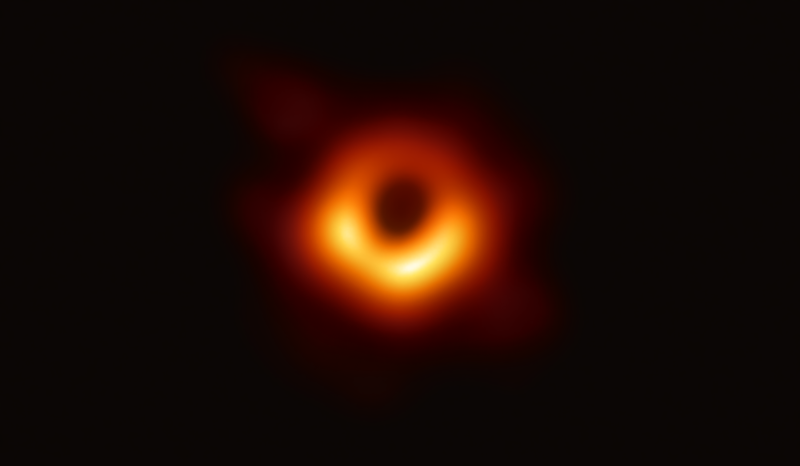
\includegraphics[width=0.5\textwidth]{20190410-78m-800x466.png}
    \caption{Fuente: \href{https://eventhorizontelescope.org/press-release-april-10-2019-astronomers-capture-first-image-black-hole}{Event Horizon Telescope}}
    \label{fig:M87}
\end{figure}

Despues de analizar todos los datos la imagen final es esta (Fig: \ref{fig:M87}).

\subsubsection{Modelo Teórico}
Antes de la observación se modelizó la imagen de M87* usando simulaciones GRMHD, los cuales consideran un caliente, turbulento y magnetizado disco orbitando un agujero negro de Kerr, que producen un poderoso jet, las simulaciones también predicen una sombra y un anillo de emisión asimétrico.\cite{event2019firstI}

\begin{figure}[H]
    \centering
    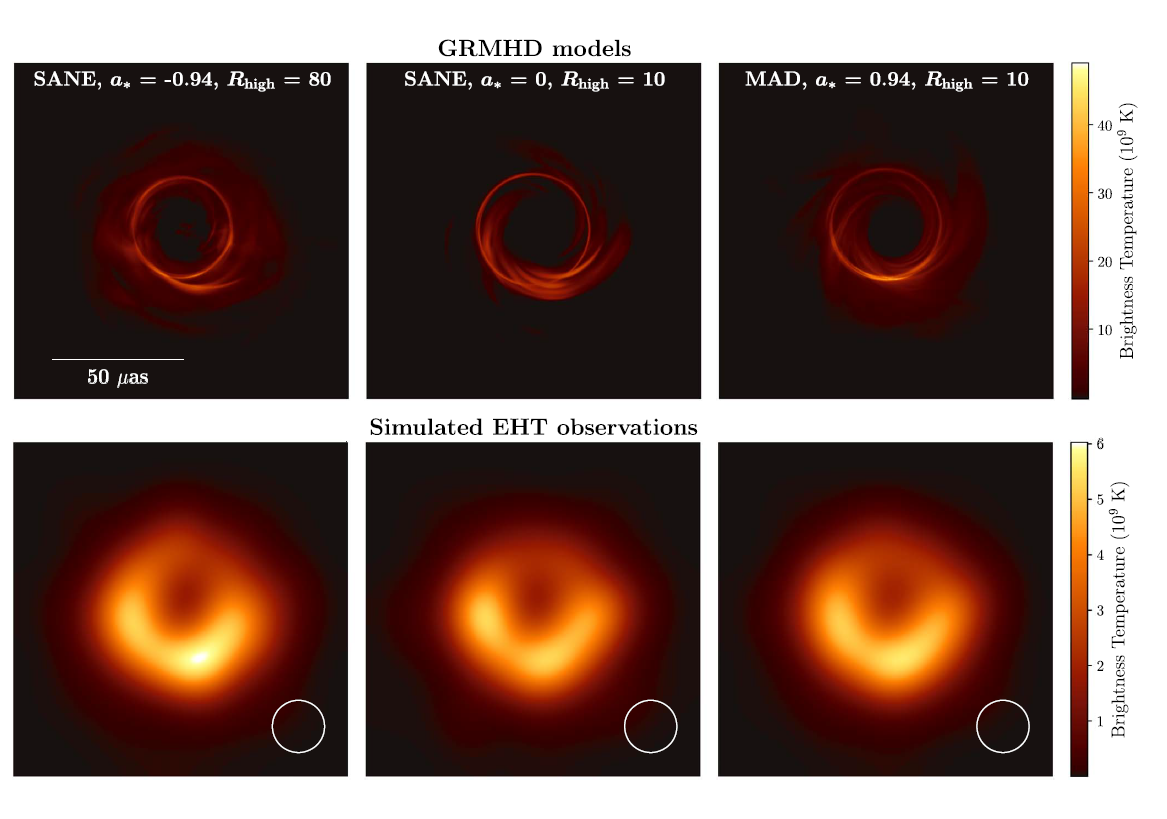
\includegraphics[width=0.5\textwidth]{M87_real_simulation.png}
    \caption{Comparación de los modelos teóricos con la imagen real, fuente: \cite{event2019firstI}.}
    \label{fig:M87_real_simulation}
\end{figure}

En (Fig: \ref{fig:M87_real_simulation}) se ve perfectamente que la simulación previa predice con mucha precisión la imagen obtenida.

\section{Conclusiones}
\section{Apéndice}
\bibliographystyle{unsrt}
\bibliography{sample}
\printindex
\end{document}